\chapter{接口使用约束描述方法研究}
\label{cha:impsec}
随着软件规模的提升与开源社区的蓬勃发展,
开发者经常利用现有的应用编程接口(API)来快速构建系统。
在使用API完成特定功能时,
需要满足对应的约束条件。
例如:参数的有效性,正确的调用序列等等。
违反这些约束中的一条或多条,
则会产生接口误用(API misuse),
导致程序错误、系统崩溃,甚至被攻击者利用。
对接口使用约束进行描述,
是避免接口误用的前提条件。
接口行为规约描述语言(BISL)提供面向代码层次的形式化描述方法,
能够有效地帮助开发者理解API的行为以及使用时需要满足的约束条件。
因此,研究面向接口使用特点的规约描述语言具有重要意义。


本章首先针对不同领域的开源C程序中接口误用缺陷实例进行分析,
总结常见缺陷模式以及违反的约束条件。
接着基于缺陷模式,提出用于描述C程序接口使用约束的领域特定语言IMSpec,
并对语言的设计动机进行介绍,定义该语言语法和语义。
本章将IMSpec应用于实际项目中的接口实例,以验证语言的有效性。
从全文的研究体系上看,本章的工作旨在通过形式化的方法对接口使用约束描述,
是接口缺陷检测工作的重要基础。


\section{引言}
开发者在使用API构造软件系统时,
需要满足特定的使用约束条件以正确地完成相应的功能。
例如:API参数为指针类型时,该指针不可以为空,
否则可能会产生一个空指针解引用错误;
当通过内存管理接口申请内存资源后,需要使用相应的释放接口以归还资源,
否则将产生一个内存泄漏错误。
这些由于误用API而产生的缺陷是软件错误、系统崩溃的重要原因之一,
甚至会被攻击者利用,带来巨大影响。


为保证API的正确使用,
一方面,API的设计者提供各种各样的文档、应用案例,
以帮助使用者理解API的功能和对应的使用约束条件。
然而,现在的文档形式难以满足实际需求~\cite{09-icse-doc}。
更严重的是,随着开源软件的蓬勃发展,
大量的软件库没有完整的文档资料,
甚至没有或者存在错误的使用说明~\cite{15-ieee-doc-fail, 17-icse-api-doc}。
同时,相对于直接查找官方的API使用文档,
更多的开发者通过网络搜索来快速地找到相应的使用方法。
但是网络资源的可靠性难以保障~\cite{18-icse-stack}。
另一方面,研究人员通过缺陷检测的方法对API误用进行查找,
以提高代码质量。
然而,现有的检测方法难以满足实际需求。
基于静态分析技术的检测工具,
多通过预先实现的检测器来进行缺陷查找~\cite{15-coufless-static-survey}。
因此,该方法难以找到未预先定义的接口误用缺陷。
基于数据挖掘技术的方法,通过推理API使用约束,
再基于这些约束来进行缺陷检测。
然而,现有的数据集质量难以满足学习算法的数据要求~\cite{survey18}。
因此,
无论是API的设计人员还是缺陷检测的研究人员,
如何有效地定义API使用约束是保证接口正确使用的重要基础。

BISL提供面向代码级别的形式化描述方法,
能够有效地帮助程序员理解API的行为以及使用中需要满足的约束条件~\cite{survey12}。
通俗来说,这些规约描述为接口的开发者和使用者提供一种形式化的契约模式(software contract)~\cite{92-ieee-contract},
即这些规约描述通过形式化的表达形式描述API在使用时需要满足的特定约束条件。
然而,针对于API使用约束的描述,
现有的BISL具有若干不足:
(1)针对普适性程序特征的BISL多面向接口实现而设计,
有利于描述API的内部属性。
随着软件的规模和复杂性增加,API的使用情景复杂化。
普适性BISL难以描述API使用约束条件,即易用性不足。
(2)针对接口使用约束的BISL通常为某个特定领域的接口而设计,
语言表达能力不足,难以应用到普适性API使用约束条件,即完备性不足。
例如:SLIC~\cite{01-slic}针对于Windows驱动程序设计,
SSLINT~\cite{15-sp-sslint}针对于SSL协议中十余个核心接口设计。


为解决上述方法中的不足,本章提出IMSpec领域特定语言(DSL),
一个基于缺陷模式的C程序接口使用约束描述语言。
首先,为能够深入理解C程序接口误用缺陷的特点从而总结接口使用约束模式,
本章以不同领域、广泛使用的六个开源软件为对象,
对近五年来830个实际接口误用实例进行分析。
本文共总结出三大类常见接口缺陷模式:
(1)不正确的参数使用(Improper Parameter Using, IPU),
(2)不正确的异常处理(Improper Error Handling, IEH),
(3)不正确的因果调用关系(Improper Causal Calling, ICC)。
这些缺陷模式一方面可以为描述语言的设计提供基础,
简化语言的复杂度。
另一方面,有利于辅助研究人员和开发者理解实际项目中的缺陷模式,
从而提高接口设计以及避免接口误用。
基于接口误用缺陷模式,本章提出面向C程序接口使用约束的领域特定语言IMSpec。
本章对IMSpec的设计原则进行介绍,并定义语法结构与形式化语义。
最后,本章将IMSpec应用于调研中发现的典型缺陷实例中,
以评估该语言的描述能力和有效性。
结果显示,IMSpec能够支持调研实例中90.67\%的接口使用约束,
%平均每个实例4.35行,
对接口使用约束具备描述能力。
同时,基于IMSpec描述与自然语言描述的接口使用约束,
本文通过调查问卷的方式邀请实际开发者来对误用实例检测的来评估IMSpec的有效性。
实验结果显示,实际开发者通过IMSpec描述的接口使用约束能够多找到43.7\%的缺陷,
即IMSpec能够有效地对接口使用约束进行描述。


本章其余部分组织结构如下:
\ref{sec:2.2}节对相关研究进行总结;
\ref{sec:2.3}节给出接口误用缺陷调研的方法并总结调研结果;
\ref{sec:2.4}节给出IMSpec的设计思路,定义语言的语法结构与形式化语义;
\ref{sec:2.5}节对IMSpec进行实际案例应用与评估;
最后在\ref{sec:2.6}节总结本章工作。

\section{相关工作}
\label{sec:2.2}
本章相关的研究包括两个方面:
接口使用相关的调研工作与规约描述语言的设计工作。
本节将分别对这两方面内容进行总结。

\paragraph{接口使用调研}
过去的二十年内,研究人员对接口使用从不同角度开展大量的调研工作以保证其被正确使用
~\cite{16-icse-cry,17-tse-survey, 12-fse-parallel,12-fse-deprecation,	18-sqj-evolution,11-etaps-doc, 15-ese-evolution, 11-ese-learning, 15-tse-change,13-etaps-mapping}。
一方面,研究人员从API设计和实现入手,
对API文档~\cite{12-fse-deprecation, 18-sqj-evolution,11-etaps-doc}、
API演化~\cite{15-ese-evolution,15-tse-change}等内容进行分析;
另一方面,则从使用者的角度,对API使用中的问题进行分析~\cite{16-icse-cry,17-tse-survey,12-fse-parallel,11-ese-learning,13-etaps-mapping}。

随着软件库的更新,新的API用来替换过时的API,
以增加稳定性、提升执行时效率。
使用这些过期的API,是API误用的一种。
Robbes~\cite{12-fse-deprecation, 18-sqj-evolution}在超过2600个系统中对577个不同的API进行研究,
以分析使用过期API带来的影响。
其结果显示,虽然只有14\%的API与其他的系统模块相关,
但是在升级后这些改变会带来极大的影响。
其中最多的一个API实例涉及到80个开发者和120个项目。
然而,很多开发者对此并没有做出相应的更新措施,
极大地降低系统的可靠性。

从使用的角度,Zhong~\cite{17-tse-survey}针对于不同类型API的使用情况进行调研分析。
从规约挖掘技术的需求,
共总结出9个与API使用相关的发现。
特别地,该论文指出在对API使用进行规约描述时,
需要考虑非顺序调用关系、类型信息和顺序关系三个特点。
同时,随着多核处理器的发展,开发人员可以利用并行化技术来加快问题求解。

Okur~\cite{12-fse-parallel}对655个开源项目中并行计算软件库中的API使用情况进行分析。
结果显示,超过10\%的开发者误用这些API,导致程序并没有并行化运行,而是在串行执行。
同时,由于对API使用约束的生疏,开发者撰写的代码复杂度高,难以理解与维护。

与Okur的工作类似,Nadi~\cite{16-icse-cry}针对加密算法的API使用情况进行分析。
该研究针对100个StackOverflow的问题与回答、100个Github上的开源项目和48个实际开发者进行调研。
其结果显示,尽管开发者认为这些API使用难度大,但是他们依旧坚信能够正确使用这些接口。
然而,在实际项目中加密算法相关API误用却普遍存在~\cite{13-ccs-misuse}。

Robillard~\cite{11-ese-learning}从开发者的角度对API使用进行调研。
通过多阶段调研问卷与面对面讨论的方式,
该研究发现开发者普遍认为API学习难度大。
其主要原因是现有的文档形式难以有效地帮助使用者理解如何正确使用接口。
特别地,缺少足够的使用样例是文档最大的不足。
因此,虽然API的设计者提供格式良好的文档,
但是开发者多利用网络资源以快速地掌握API的使用情况。
%这也对缺陷检测后的结果展示提出要求。

现有的接口使用调研工作多针对面向对象编程语言展开~\cite{16-icse-cry,17-tse-survey, 12-fse-parallel,12-fse-deprecation},
因此其结果难以直接应用于C程序。
针对接口误用缺陷,Okur对并行化API的缺陷模式进行分析,
同时Nadi对加密算法相关的API使用情况进行分析。
这些方法都只针对于某一个特殊领域,其结果难以直接适用于普适性接口误用缺陷模式。


\paragraph{规约描述语言}
软件行为规约(behavorial specification)是对软件系统或者组件预期行为的精确描述。
独立的代码实现并不能有效描述其功能和使用约束,
因此通过规范形式记录下来的信息对于软件维护有着重要作用,
能够有效地描述API开发者和使用者之间的协议~\cite{92-ieee-contract}。
特别地,形式化规约描述语言能够消除自然语言的歧义。
规约能够在软件的整个开发周期使用,
一方面开发人员可以根据规约进行内部功能实现;
另一方面测试人员能够在调试阶段根据规约去分离错误,划分责任~\cite{05-vstte-spec}。
近三十年来,研究人员针对不同的语言和目标,设计并实现了各种各样的BISL~\cite{survey12}。
例如,针对通用属性检测的BLAST~\cite{blast}、ACSL~\cite{acsl};
针对领域特定的BISL包括:SSL协议的SSLINT~\cite{15-sp-sslint}、
Windows内核驱动程序的SLIC~\cite{01-slic}、Epex工具中对异常处理检测的规约~\cite{16-sec-epex}等等。


BLAST~\cite{blast}由Dirk Beyer教授提出,是面向时序安全属性的规约描述语言,
用于BLAST自动化验证工具。
该语言从两个不同的精度水平对程序属性进行描述。
微观来说,该语言能够通过描述检测自动机(monitor automata)的内部转移,
在程序的运行时轨迹上对程序时序属性进行分析。
宏观来讲,该语言通过撰写可达性查询语句,
对程序的状态与位置进行查询。
通过两个精度水平的描述,BLAST能够有效地将验证问题转化到多个独立的模型检测引擎中,
从而降低验证工作的复杂性。

ACSL(ANSI/ISO C Specification Language)是Frama-C~\cite{16-rv-framac}代码分析平台用来形式化定义C程序属性的规约描述语言。
该语言通过注释的方式对程序中属性进行描述,以辅助验证工具对代码实现情况进行检测。
ACSL注重函数合约(function contract),
即函数的参数与函数执行后需要满足的性质。
其中,前者也被称作前置条件(pre-condition);后者被称作后置条件(post-condition)。
特别地,前置条件多针对于API使用者,即在调用目标API之前需要满足的约束。
ACSL以代码注释的形式撰写,因此为利用ACSL,
分析工具需要理解ACSL的语法与语义,同时将ACSL与目标C程序的源代码进行转化。


针对于C程序接口误用缺陷检测,微软公司SLAM项目~\cite{slam}是典型代表之一。
开发者通过使用SLIC规约描述语言~\cite{01-slic}对程序接口的属性进行描述,
并使用基于反例引导抽象解释技术的SDV验证工具对目标API使用情况进行检查。
至2010年,该项目已经积累超过200个API使用规约,
成功检测到Windows操作系统驱动程序中270个API误用缺陷,
有效提高接口使用的正确性~\cite{10-cad-slam, 11-acm-slam}。
此外,SSLINT基于程序依赖图(program dependency graph)对SSL安全相关的API进行建模
并通过Cypher~\cite{18-sigmod-cypher}图查询语言对预定义好的模式进行查询,
以检测API误用。
Epex对API返回值的约束条件进行描述,
并利用规约对C程序中接口执行失败后不正确的异常处理代码进行检测。

现有规约描述语言对于C程序接口使用约束的描述存在若干不足。
一方面,通用语言针对多种程序属性设计,通常为接口功能实现而设计,语法结构多样,语义丰富。
然而,接口使用多含有复杂的程序结构,涉及到多个API的协同使用。
因此通用语言描述使用约束需要复杂的组合。
另一方面,现有针对接口使用的描述语言多针对某个特定领域或者某些接口实例设计,
难以扩展到普适性的接口使用约束。
例如SLIC语言能够有效的应用于Windows操作系统驱动程序,
却难以应用于SSL安全库中的接口。


\section{接口误用缺陷分类}
\label{sec:2.3}
为能够在实践中更加有效地解决API误用问题,
对API误用缺陷的特点进行深入研究以总结API使用约束具有重要意义。
针对于接口误用缺陷模式,
一方面,可以通过现有缺陷分类标准进行总结;
另一方面则可以通过现有接口误用缺陷检测研究中的缺陷模式进行概括与总结。

IEEE组织在1993发布IEEE-1044软件异常分类,并在2009年更新~\cite{09-ieee-classification}。
基于该标准的内容,IBM公司提出Orthogonal Defect Classification(ODC)分类标准~\cite{92-tse-odc}。
ODC基于缺陷类型(defect type)对缺陷进行分类,
即通过代码结构的组成进行分类。
例如函数、检测、赋值、文档等等。
%一个缺陷类型具体可以表现为两种异常类型(violation type),即缺失或者误用。
2016年Beller~\cite{16-saner-evaluation}基于ODC提出General Defect Classification(GCD),
从而更加精确地比较静态分析技术的检测能力。
然而现有的缺陷分类方式,一方面没有对所有的软件缺陷类型进行描述,因此无法涵盖所有接口误用缺陷域;
另一方面缺少对API误用缺陷的详细分类情况。

过去的十几年内,研究人员对不同的接口误用缺陷模式进行检测。
例如,Monperrus~\cite{13-tosem-missing-call}指出,
缺失必要的API调用普遍存在于缺陷跟踪系统、论文和源代码以及代码的注释中。
Thummalapenta~\cite{09-icse-exception}针对API调用前需要满足的前置条件进行研究。
Wasylkowski~\cite{07-fse-object}则对接口调用顺序相关错误进行检测。
然而,这些研究都只针对接口误用缺陷中某一个特定的种类。
Adama~\cite{survey18}在其研究结果中针对Java程序提出API-Misuse Classification(MUC),
从而对API误用缺陷进行分类,并比较现有工具的检测能力。
该分类基于API使用元素与缺陷表现类型进行分类。
一个缺陷类型具体可以表现为两种异常类型(violation type),即缺失(missing)或者误用(misuse)。
本文针对C程序的API缺陷进行研究,C程序与Java程序存在巨大设计理念差异。
该结果难以直接应用于本文研究内,但是对本文的研究具有重要参考意义。
另一方面,研究人员从API使用本身入手,
调研并总结面向API使用说明性质的(directive)分类~\cite{09-icse-doc,12-ese-directive}。
API使用说明,是API文档中的一段自然语言描述,
可以用来提醒开发者在使用API时需要满足的约束条件。
当这些约束条件被使用者忽略或者违反时,认为使用者产生一个API误用。
然而只有部分说明可以直接对应于接口误用以及产生的缺陷,其他的则更注重API的内部功能或者特殊用法。
例如:明确地说明API的参数可以为空是针对API使用中不同方式的引导。
不过这些调研结果可以作为本文的重要参考内容。


据本文调研结果显示,目前并没有研究工作对C程序接口误用缺陷的问题域进行定义或描述。
因此,研究人员难以直接对现有研究进行系统的了解与总结。
特别是哪些API缺陷种类已经被研究过和哪些没有被研究过,
以及现有的方法能够解决多少问题和方法之间的效果比较。
因此,为更好的应对C程序API误用缺陷检测以及接口使用约束描述语言的设计,
我们需要一个来源于实际程序、具有接口使用特定领域的缺陷类别。
本节剩余部分将对数据收集和分类结果进行详细描述,
并对接口缺陷分类调研结果进行讨论。

\subsection{数据收集}
本小结将针对数据收集的主要步骤进行详细描述,
包括研究对象、缺陷实例收集方法和缺陷分析方法。

\paragraph{研究对象}
\begin{table}[t]
	\centering
	\begin{minipage}[t]{0.9\linewidth} % 如果想在表格中使用脚注,minipage是个不错的办法
		\caption{API误用缺陷研究对象。}
		\label{tab:2-3-target}
		\begin{tabular}{lp{3cm}<{\centering}p{3cm}<{\centering}p{4cm}<{\centering}}
			\hline
			{\heiti 研究对象} & 
			\multicolumn{1}{c}{\heiti 关注数\footnote{本文选取Github上Watch和Star中较多者。}} &
			\multicolumn{1}{c}{\heiti 提交次数} & 
			\multicolumn{1}{c}{\heiti 可用时间\footnote{Github上可以追溯的代码修改时间。}} \\
			\hline
			Linux内核   & 69,697 & 812,391 & 20050416-至今\\
			OpenSSL   & 9,510 & 23,412 & 19981221-至今\\
			FFmpeg   & 13,907 & 93,218 & 20001220-至今\\
			Curl   & 24,009 & 12,130 & 19991229-至今\\
			FreeRDP   & 2,959 & 13,030 & 20110630-至今\\
			Httpd   & 2,028 & 31,341 & 19960703-至今\\
			\hline
		\end{tabular}
	\end{minipage}
\end{table}


当代软件开发模式多利用开源社区已有的实现对功能进行封装,
因此对开源软件的研究具有重要意义。
为能够更好地理解现实中C程序API误用缺陷的特点以及开发者如何对这些缺陷进行修复,
本文对不同领域、广泛使用的六个开源软件进行分析。
如表\ref{tab:2-3-target}所示,
这六个项目为:
\begin{enumerate}
	\item Linux内核~\cite{linux}:
	Linux内核是一种开源的类Unix操作系统内核,由芬兰赫尔辛基大学学生Linus Torvalds于1991年创建。
	该内核由一系列的程序组成,包括中断服务程序、负责管理多个进程从而分享处理器时间的调度程序、
	负责管理地址空间的内存管理程序、网络、进程间通信的系统服务程序等。
	随着开源社区的发展、软件日益复杂的功能和各种硬件的发展,越来越多的驱动程序被集成在Linux内核中。
	Linux内核在近年来发展迅速,代码量已经超过13MLOC。
	
	\item OpenSSL~\cite{openssl}:
	安全套接层协议(SSL)可以在网络上对传输内容进行加密,以提供秘密性传输的功能。
	OpenSSL则是实现该协议的开源软件库。
	该库提供三个主要的功能模块:SSL协议库、密码算法库以及应用程序。
	OpenSSL提供强大和全面的功能,囊括主要的密码算法、常用的密钥和证书封装管理功能以及SSL协议,
	并提供丰富的应用程序供测试或其它目的使用。
	应用程序可以使用OpenSSL进行安全通信,避免窃听。
	
	
	\item FFmpeg~\cite{ffmpeg}:
	FFmpeg是一套针对多媒体处理的开源软件库与应用程序的集合,
	可以用来记录和转换数字音频、视频,
	并能将数字媒体转化为流数据。
	该库由若干子项目组成,包括:多媒体编码解码算法、
	公用工具函数库、视频场景处理库、
	后期效果处理库、格式转换、基于HTTP多媒体即时广播串流服务器以及
	多媒体播放器等等。
	
	\item Curl~\cite{curl}:
	Curl是一个利用URL语法~\cite{url},在命令行下工作的文件传输工具。
	该工具支持文件的上传和下载,被称作为综合传输工具。
	Curl支持多种通信协议,同时还提供多种安全验证机制。
	自1997年首次发行以来,该工具被开发者广泛应用,吸引上千开发者的贡献。
	已经成功应用于汽车、电视、交换机、打印机、手机、平板电脑等多个领域。
	同时,Curl还提供libcurl接口库供程序员开发使用。
	
	\item FreeRDP~\cite{freerdp}:
	远程桌面协议(Remote Desktop Protocol,RDP)是一个多通道的远程连接协议,
	能够让客户端连接到提供远程服务的Windows服务机。
	FreeRDP是一款基于Apache协议实现RDP的开源软件。
	目前该软件已经成功应用于多个Linux发布版以及Mac系统。
	
	
	\item Httpd~\cite{httpd}:
	Httpd是Apache开源组织研发面向超文本传输协议(HTTP)服务器的主程序。
	该程序以独立运行的后台进程存在,并通过子进程或者线程池形式对请求进行处理。
	Httpd代码开源,并被广泛应用于各种网络服务中,
	目前已经成为网络上最受欢迎的服务器之一。
	
\end{enumerate}

上述研究对象涵盖不同的领域:操作系统(Linux内核),开源API库(OpenSSL和FFmpeg),
Ubuntu应用软件(Curl,FreeRDP和Httpd)。
具有多年的开发历史,并且现在依旧活跃于开源社区中,
被应用人员广泛使用。
一方面,活跃的开发者和用户社区有利于缺陷的报告和修复;
另一方面,被广泛使用使得这些软件的代码质量更具有代表性。
特别是针对于代码质量,
大量的使用者和开源社区贡献能够快速地对程序中的缺陷进行修复。
同时,这些项目都在Github网站上开源、具有完整的修改记录和缺陷跟踪系统。
这些修改记录和缺陷跟踪系统有利于缺陷实例的收集和总结。
因此,本文选择以上项目作为分析对象。
%为方便研究人员和开发者进行扩展、研究其他领域问题,
%本文将数据抽取的工具和方法公布于。

\paragraph{缺陷实例收集}
\begin{table}[t]
	\centering
	\begin{minipage}[t]{0.9\linewidth} % 如果想在表格中使用脚注,minipage是个不错的办法
		\caption{API误用缺陷研究对象}
		\label{tab:2-3-statistics}
			\begin{tabular}{crcrrr}
			\hline
			\multirow{2}{*}{项目名称} & \multirow{2}{*}{Loc} & 研究 & \multicolumn{1}{c}{修改}& \multicolumn{1}{c}{缺陷}& \multicolumn{1}{c}{API误用}\\
			&  & 时间 & \multicolumn{1}{c}{总数} & \multicolumn{1}{c}{数目}& \multicolumn{1}{c}{数目} \\
			\hline
			Linux & 12.96M & 20170901-20171231 & 24651 & 6401 & 868 \\
			%\hline
			OpenSSL & 454K & 20150701-20171231 & 7564 & 2391 & 529 \\
			%\hline
			FFmpeg & 915K & 20160701-20171231 & 8162 & 2783 & 610 \\
			%\hline
			Curl & 113K & 20130101-20170630 & 7082 & 2043 & 499 \\
			%\hline
			FreeRDP & 259K & 20130701-20171231 & 7565 & 3535 & 495 \\
			%\hline
			Httpd & 203K & 20130701-20171231 & 6072 & 1323 & 149 \\
			\hline
			Total & 14.90M & - & 61096& 18476 & 3150 \\
			\hline
		\end{tabular}
	\end{minipage}
\end{table}


本文通过对软件开发版本修改记录日志分析,以完成API误用缺陷实例收集工作。
如表\ref{tab:2-3-statistics}所示,本文在六个开源项目中,
共对61096个修改记录进行分析,在18476个缺陷修复记录中收集3150个API误用缺陷实例。
下文将详细描述缺陷实例的收集方法。

首先,通过Github上的日志记录追踪系统,对所有的修改记录进行下载和备份。
针对于每一次修改记录,抽取修改说明(description)、
修改的差异性报告(diff文件)以及修改前和修改后的源代码文件。
图\ref{fig:2-3-description}给出Linux内核修改sha:059c98599的修改说明,
包括:修改的哈希值、概要总结、详细说明、作者、时间以及上一版本的哈希值。
根据本次修改的哈希值以及上一修改的哈希值,可以抽取(checkout)相应版本的源文件,
即修改前和修改后的文件。
图\ref{fig:2-3-diff}给出该修改的差异性报告。
其中以“+”开始的绿色行为增加的行,以“-”开始的红色行为删除的行。

\begin{figure}[t]
	\centering
	\begin{minipage}{0.75\linewidth}
{\footnotesize	
%\begin{lstlisting}
"hash": "059c98599b1ab1e2e479e1f4617948d4c2a32b84",\\
"summary": "wl18xx: add checks on wl18xx\_top\_reg\_write() return value",\\
"description": 
"wl18xx: add checks on wl18xx\_top\_reg\_write() return value.
Check return value from call to wl18xx\_top\_reg\_write(),
so in case of error jump to goto label out and return.
Also, remove unnecessary value check before goto label out.\\
Addresses-Coverity-ID: 1226938\\
Signed-off-by: Gustavo A. R. Silva <garsilva@embeddedor.com>\\
Signed-off-by: Kalle Valo <kvalo@codeaurora.org>",\\
"date": "2017-06-28 21:18:40",\\
"author": "Gustavo A. R. Silva",\\
"parent\_hash": "69551f5f370cc20342fab17ca54716b6ec7e332d"	
%\end{lstlisting}
}
	\end{minipage}
	\caption{
	Linux内核修改sha:059c98599的修改说明。
	}
	\label{fig:2-3-description}
\end{figure}
\begin{figure}
	\centering
\begin{lstlisting}
drivers/net/wireless/ti/wl18xx/main.c
=======================================================
lhs: 100644 | d1aa3eee0e81f8cc7612eddabc4cf630dbbd1e79
rhs: 100644 | 0cf3b4013dd646104b1f153c3d8a191f12a5dba8
@@ -793,9 +793,13 @@ static int wl18xx_set_clk(struct wl1271 *wl)
ret = wl18xx_top_reg_write(wl, PLLSH_WCS_PLL_P_FACTOR_CFG_2,
	(wl18xx_clk_table[clk_freq].p >> 16) &
	PLLSH_WCS_PLL_P_FACTOR_CFG_2_MASK);
+		if (ret < 0)
+			goto out;
} else {
ret = wl18xx_top_reg_write(wl, PLLSH_WCS_PLL_SWALLOW_EN,
	PLLSH_WCS_PLL_SWALLOW_EN_VAL2);
+		if (ret < 0)
+			goto out;
}

/* choose WCS PLL */
@@ -819,8 +823,6 @@ static int wl18xx_set_clk(struct wl1271 *wl)
/* reset the swallowing logic */
ret = wl18xx_top_reg_write(wl, PLLSH_COEX_PLL_SWALLOW_EN,
	PLLSH_COEX_PLL_SWALLOW_EN_VAL2);
-	if (ret < 0)
-		goto out;

out:
return ret;

\end{lstlisting}
	\caption{
	Linux内核修改sha:059c98599的差异性报告。
	}
	\label{fig:2-3-diff}
\end{figure}

接着对修改记录进行分析,抽取本文关心的接口误用缺陷实例。
如表\ref{tab:2-3-statistics}所示,在六个项目中,本文共获得61096个修改记录实例。
由于不同的领域背景、代码的复杂性、接口的熟悉程度等原因,
在现阶段情况下,针对每一个实例进行分析难以完成。
因此本文通过自然语言处理的方式,在修改说明中对接口误用缺陷进行提取:
\begin{enumerate}
	\item 针对六个项目,本文随机在每一个项目中选择100个修改记录实例进行详细分析。
	通过API文档研究、代码查看、开发者讨论等方式,本文筛选出与缺陷修复(bug fix)相关的实例,
	并总结这些实例中与缺陷修复相关的关键词。
	例如:“bug”,“error”,“fix”和“check”等等。
	\item 在缺陷修复相关的实例中,进一步筛选和API误用缺陷相关的实例。
	本文利用在已发表论文中的缺陷类型以及其他针对软件缺陷分类中的类型作为基础,
	对缺陷的原因进行判断。
	如果缺陷的产生原因出现在上述分类中的一种或者多种,或者是违反官方文档中接口使用约束,
	那么就认为这是一个API误用缺陷。
	本文对这些缺陷修改描述中的关键词进行总结,
	例如:“fix API”,“missing check”,“null pointer dereference”,“add check” “memory leak”以及“return value”等等。
	\item 基于这些关键词本文在已经提取的61096个缺陷实例中基于自然语言处理的方式进行文本匹配,
	通过筛选缺陷修改说明来获取目标研究对象中的缺陷实例。
	对于选中的结果,本文过滤掉所有没有修改过*.c源文件的修改记录。
\end{enumerate}

图\ref{fig:2-3-description}和图\ref{fig:2-3-diff}是一个缺陷实例。
在Linux项目中,通过关键词的搜索,本文认为修改sha:059c98599的修改与缺陷修复有关。
因为修改的描述中包含关键词“check”,即“\underline{Check} return value from call to wl18xx\_top\_reg\_write()”。
此后在API误用缺陷实例的搜索过程中,
该修改还包括“\underline{add checks} on wl18xx\_top\_reg\_write() return value”。
因此,本文认为该修改与接口缺陷相关。
如图\ref{fig:2-3-diff}所示,该修改用来修复不正确的API返回值检查缺陷。
该缺陷的原因以及缺陷模式将在后文中进行详细分析。

针对于该方法的有效性,本文在抽取的结果中通过随机取样进行验证。
在所有提取的API误用缺陷修复实例中,本文在每个项目中随机选择30个样例。
通过对这180个实例的详细分析,发现其中166个是API误用缺陷修复实例,
即准确率达到92.22\%。
在所有的误报实例中,虽然修改说明中出现相应的关键词,
但是修改的内容本身与API误用无关。
例如:OpenSSL的一个修改记录sha:4af389为“Fix compilation with OPENSSL API compat”。
该描述中包含“fix API”关键词,然而,该修改针对于编译错误。
因此,本文认为通过以上方法能够有效地在修改记录中获取API误用缺陷实例。

在预实验阶段,由于缺少领域知识、对API掌握熟练度不足、以及缺陷的复杂性,
平均每个缺陷的理解时间在3.5小时。
特别地,有的缺陷报告涉及多个文件,包含API缺陷修改、重构、文档等多个内容。
现阶段情况下难以在有限的时间内,针对每一个实例进行详细分析。
因此,本文在3150个API误用缺陷实例中,
在每个项目中抽取35\%的缺陷实例进行详细分析。
针对于这部分缺陷,进一步将修改超过两个文件、修改行数大于30行的修改记录进行过滤。
如表\ref{tab:2-3-studied}所示,最终本文在3150个API缺陷实例中,
对随机抽取的830个缺陷实例(26.35~\%)进行深入分析。

\begin{table}[t]
	\centering
	\begin{minipage}[t]{0.85\linewidth} % 如果想在表格中使用脚注,minipage是个不错的办法
		\caption{API误用缺陷实例统计信息}
		\label{tab:2-3-studied}
		\begin{tabular}{cccccc}
			\hline
			\multirow{2}{*}{项目名称} & \multirow{2}{*}{缺陷总数} & \multicolumn{2}{c}{API误用}& \multicolumn{2}{c}{研究实例}\\
			\cline{3-4}\cline{5-6}
			&  & 数量 & 百分比(\%)\footnote{与缺陷总数的百分比} & 数量& 百分比(\%)\footnote{与API误用缺陷总数的百分比} \\
			\hline
			Linux & 6401 & 868 & 13.56 & 283 & 32.60 \\
			%\hline
			OpenSSL & 2391 & 529 & 22.12 &127  & 24.00 \\
			%\hline
			FFmpeg & 2783 & 610 & 21.92 & 126 & 20.66 \\
			%\hline
			Curl & 2043 & 499 & 24.42 & 134 & 26.85 \\
			%\hline
			FreeRDP & 3535 & 495 & 14.00 & 119 & 24.04 \\
			%\hline
			Httpd & 1323 & 149 & 11.26 & 41 & 27.52 \\
			\hline
			总计 & 18476 & 3150 & 17.05 & 830 & 26.35 \\
			\hline
		\end{tabular}
	\end{minipage}
\end{table}
\paragraph{缺陷分析}
对于上述步骤收集的缺陷实例,本文通过修改说明文件的内容、差异性报告以及
源代码文件对缺陷进行深入理解。
包括:接口误用上下文语义中的根本原因、修复的模式以及误用的其他统计信息等。
特别地,为能够理解API误用缺陷的本质,
本文关注API误用的约束条件,即在API使用的整个代码片段中,哪一部分的错误导致API误用。

以图\ref{fig:2-3-diff}为例。
通过缺陷描述可知,
该缺陷产生的原因是没有对接口~\texttt{wl18xx\_top\_reg\_write()}的返回值进行检查。
同时,差异性报告中显示该缺陷的修复方式是增加返回值\texttt{ret}的检查,
即判断返回值是否小于零。
此外本文发现,如果小于零则添加\texttt{goto}语句,跳转至异常处理部分。
总结来说,该缺陷产生的上下文是~\texttt{wl18xx\_top\_reg\_write()}函数调用后,没有进行返回值检查;
缺陷的根本原因则是没有对该函数进行异常处理;
修复的模式则相对简单,即进行检查并在错误路径上添加跳转语句至异常处理模块。


\subsection{调研结果}
如表\ref{tab:2-3-studied}所示,
在18476个缺陷修复实例中,有3150个与API误用相关的修复实例,
平均百分比为17.05\%。
其中Curl占比例最多,为24.42\%;
Httpd最少,为11.26\%。
在上文介绍的预实验方法和结果中,平均92.22\%的API误用缺陷为真正例(True Positive,TP)。
因此,本文相信API误用缺陷并不是开发阶段发生的偶然事件,
其具有普遍性。

\vspace*{10pt}
\begin{center}
\noindent\shadowbox{
	\centering
	\begin{minipage}{0.85\textwidth}
		{\kaishu 发现1:API误用缺陷普遍存在被分析系统中。
			调研结果显示,平均17.05\%缺陷修复相关的修改记录与API误用相关。}
	\end{minipage}
}
\end{center}

为能够理解API误用缺陷的本质原因,本文对随机选取的830个缺陷实例进行分析,
包括出错的根本原因、误用缺陷的修复模式以及API误用重复发生的统计信息。
下文将对调研的结果进行仔细分析。

\begin{table}[b]
	\centering
	\begin{minipage}[t]{\linewidth} % 如果想在表格中使用脚注,minipage是个不错的办法
		\caption{API误用缺陷实例统计信息}
		\label{tab:2-3-root-causes}
		\begin{tabular}{cccccccccc}
			\hline
			\multirow{2}{*}{项目名称} & 实例 & \multicolumn{2}{c}{IPU}& \multicolumn{2}{c}{IEH}& \multicolumn{2}{c}{ICC}& \multicolumn{2}{c}{其他}\\
			\cline{3-10}
			& 个数 & 数量 & 百分比 & 数量& 百分比 & 数量& 百分比& 数量& 百分比 \\
			\hline
			Linux  & 283 & 43 & 15.1 & {96} & {33.92} & 77 & 27.21 & 67 & 23.67 \\
			%\hline
			OpenSSL  & 127 & 21 & 16.54 & 42 & 33.07 & {49} & {38.58} & 15 & 11.81 \\ 
			%\hline
			FFmpeg  & 126  &  18 & 14.29 & 43 & 34.13 & 52 & 41.27 & 13 & 10.32 \\
			%\hline
			Curl  & 134   & 23 & 17.16 & 38 & 28.36 & 57 & 42.54 & 16 & 11.94 \\ 
			%\hline
			FreeRDP   & 119 & 22 & 18.49 & 30 & 25.21 & 48 & 40.34 & 19 & 15.97 \\ 
			%\hline
			Httpd  & 41 & 8 & 19.51 & 8 & 19.51 & 16 & 39.02 & 9 & 21.95 \\ 
			\hline
			Total  & 830 & \multicolumn{2}{c}{135 (16.27\%)} & \multicolumn{2}{c}{257 (30.96\%)} & \multicolumn{2}{c}{299 (36.02\%)} & \multicolumn{2}{c}{139 (16.75\%)}\\ 
			\hline
		\end{tabular}
	\end{minipage}
\end{table}
\paragraph{根本原因}

在对所有的目标用例分析后,本文将统计结果总结于表\ref{tab:2-3-root-causes}中。
虽然每个项目中出错的根本原因分布不同,
但是可以总结出三大类常见C程序接口误用缺陷模式:
不正确的参数使用(Improper Parameter Using, IPU)、
不正确的异常处理(Improper Error Handling, IEH)、
不正确的因果调用关系(Improper Causal Calling, ICC)。
下文中将通过缺陷实例对这些缺陷类型进行讲解。

\begin{figure}[b]
	\centering
\begin{lstlisting}
"description": "Fixed API nonnull warning."
"date": "2014-11-17 00:00:09"
"author": "Armin Novak"
libfreerdp/core/gateway/http.c
=======================================================
lhs: 100644 | 4cef378c8cafdc4ad4a237f88a092c511c250ffa
rhs: 100644 | 51c5c04dc257975756a4ee3ded16cae493dea95c
@@ -330,10 +330,12 @@ void http_request_free(HttpRequest* http_request)

BOOL http_response_parse_header_status_line(HttpResponse* http_response, char* status_line)
{
-	char* separator;
+	char* separator = NULL;
char* status_code;
char* reason_phrase;
-	separator = strchr(status_line, ' ');
+
+	if (status_line)
+		separator = strchr(status_line, ' ');

if (!separator)
	return FALSE;
@@ -433,7 +435,10 @@ BOOL http_response_parse_header(HttpResponse* http_response)
*                 |     |
*         colon_pos     value
*/
-		colon_pos = strchr(line, ':');
+		if (line)
+			colon_pos = strchr(line, ':');
+		else
+			colon_pos = NULL;

if ((colon_pos == NULL) || (colon_pos == line))
	return FALSE;

\end{lstlisting}
	\caption{
	FreeRDP中空指针引用导致的IPU-API误用缺陷(sha:9e5be6f7e8)。
	}
	\label{fig:2-3-ipu-1}
\end{figure}

\noindent{\textbf{\textit{IPU}}}:软件库的开发者提供API以实现对特定功能封装,
达到软件复用的作用。
然而,开发者在使用这些API的时候,需要满足特定的约束条件,
以保证API使用时上下文环境正确。
这些API被调用前需要满足的条件,亦被称作前置条件(pre-condition)~\cite{14-fse-pre}。

例如,一个API的参数中包含指针类型,
那么通常情况下在调用该API之前,需求保证该指针不为空指针NULL。
然而,本文发现API的使用者经常忽略这些约束条件,
导致空指针解引用错误。
图\ref{fig:2-3-ipu-1}给出一个FreeRDP项目中的缺陷修改记录。
接口\texttt{strchr(str, c)}用来搜索字符串\texttt{str}中,
第一次出现字母\texttt{c}的位置。
其中\texttt{str}是一个指向字符串的指针。
在FreeRDP项目http.c文件中定义的接口\texttt{http\_response\_parse\_header\_status\_line()}中,
将来自外部输入的参数\texttt{status\_line}作为实参传递给\texttt{strchr}。
然而在调用\texttt{strchr}之前(16行与27行),并没有对该参数进行非空指针检查。
如果该参数为空指针,则会产生一个API误用,导致程序崩溃。
为避免该缺陷,开发者增加参数非空检查的条件判断,如图中18-19行与28-31行所示。


\begin{figure}[t]
	\centering
\begin{lstlisting}
"hash": "f7d183f08472e566a2e6b62a80e200a12670ed0e",
(*@\textcolor{black}{"summary": "libxvid: Check return value of write() call",}@*)
"date": "2016-11-11 10:17:07",
"author": "Diego Biurrun",
libavcodec/libxvid_rc.c
=======================================================
lhs: 100644 | eddbbe8c651407bdc85652191a7ba964c1776f74
rhs: 100644 | 94301a2ac1ffc10a8b22ba491c70013463107452
@@ -87,7 +87,10 @@ av_cold int ff_xvid_rate_control_init(MpegEncContext *s)
(rce->i_tex_bits + rce->p_tex_bits + rce->misc_bits + 7) / 8,
(rce->header_bits + rce->mv_bits + 7) / 8);

-    write(fd, tmp, strlen(tmp));
+    if (strlen(tmp) > write(fd, tmp, strlen(tmp))) {
+        av_log(s, AV_LOG_ERROR, "Cannot write to temporary pass2 file.\n");
+        return AVERROR(EIO);
+    }
}

close(fd);

\end{lstlisting}
	\caption{
	FFmpeg中参数、返回值关系的IPU-API误用缺陷(sha:f7d183f084)
	}
	\label{fig:2-3-ipu-2}
\end{figure}
此外,接口参数之间、参数与返回值之间的语义关系也需要考虑。
最典型的就是C标准库中内存操作相关的接口。
例如,接口\texttt{memcpy(d, s, n)}用来从源内存区间\texttt{s}中,
拷贝\texttt{n}个字符到目标内存区间\texttt{d}。
因此,该函数在使用的时候,目标内存区间\texttt{d}的大小要大于或者等于拷贝长度\texttt{n}。
否则将产生一个内存越界错误。
另一方面,参数与返回值之间也可能存在语义关联关系。
例如,接口\texttt{size\_t write(int fd, void* buf, size t cnt)}从参数\texttt{buf}指向的内存区域内,
读取\texttt{cnt}个字符到参数\texttt{fd}所标志的文件或者网络链接(socket)。
该接口的返回值记录实际输出字节个数。
特别地,\texttt{write()}的返回值为负数表明该函数调用发生错误。
因此如果需要确保\texttt{cnt}个字节被写入到目标地址时,
需要显式地检查该值与函数的返回值之间的数值关系。
然而如图\ref{fig:2-3-ipu-2}中13行所示,
FFmpeg项目中libxvid\_rc.c文件在调用该接口后并没有对返回值与参数进行比对,
从而忽略API参数与返回值之间的约束关系。
为避免该错误,开发者增加返回值与参数之间的约束关系检查,如图中14-17行所示。

\vspace*{10pt}
\begin{center}
	\noindent\shadowbox{
		\centering
		\begin{minipage}{0.85\textwidth}
			{\kaishu 发现2:在所有被研究的API误用缺陷实例中,14.29-19.51\%缺陷产生的原因是
				不正确的参数使用(Improper Parameter Using,IPU),
				包括缺失或者错误地对单个参数属性、参数之间以及参数和返回值之间的约束检查。
			}
		\end{minipage}
	}
\end{center}


\noindent{\textbf{\textit{IEH}}}:
安全可靠的软件需要对所有可能出错的条件进行捕获,
并对捕获的异常进行对应的处理。
因此,高阶(high-level)编程语言多提供一套完整的异常处理机制,
以保证即使底层的功能出错,系统整体也能够正常处理不会崩溃。
不幸的是,C语言并没有提供原生的异常处理机制。
所以,在C程序中开发者需要自己定义这样的异常处理机制。
由于缺少统一的处理方式,异常处理代码经常和项目的领域特定信息相关,
形式多样、重复性高、代码繁琐等等。
特别地,当函数调用发生错误后,未能正确进行异常处理则会产生异常处理缺陷,
甚至会导致严重的安全漏洞,
例如:CVE-2014-0092~\cite{CVE-2014-0092},CVE-2015-0208~\cite{CVE-2015-0208},
CVE-2015-0285~\cite{CVE-2015-0285},CVE-2017-3318~\cite{CVE-2017-3318},
CVE-2017-5350~\cite{CVE-2017-5350}等等。
事实上,根据开源网络应用安全项目(The Open Web Application Security Project)指出,
不正确的异常处理是导致软件安全漏洞的十大因素之一~\cite{07-owasp}。

\begin{figure}[t]
	\centering
\begin{lstlisting}
"hash": "086ad79970f3cd0463558bfb69122f6acdc9d2da",
"summary": "ldap: check Curl_client_write() (*@\textcolor{black}{return}@*) codes",
"date": "2014-12-10 00:41:32",
"author": "Daniel Stenberg",
ib/ldap.c
=======================================================
lhs: 100644 | 14437c3b54715cb5ad161d78ee7b89a412b64a9d
rhs: 100644 | 96521bf21862540e32368e229365ed49d6f43cff
---@@ -384,9 +384,17 @@ static CURLcode Curl_ldap(struct connectdata *conn, bool *done)
char  *dn = ldap_get_dn(server, entryIterator);
int i;

-    Curl_client_write(conn, CLIENTWRITE_BODY, (char *)"DN: ", 4);
-    Curl_client_write(conn, CLIENTWRITE_BODY, (char *)dn, 0);
-    Curl_client_write(conn, CLIENTWRITE_BODY, (char *)"\n", 1);
+    result = Curl_client_write(conn, CLIENTWRITE_BODY, (char *)"DN: ", 4);
+    if(result)
+      goto quit;
+
+    result = Curl_client_write(conn, CLIENTWRITE_BODY, (char *)dn, 0);
+    if(result)
+      goto quit;
+
+    result = Curl_client_write(conn, CLIENTWRITE_BODY, (char *)"\n", 1);
+    if(result)
+      goto quit;

\end{lstlisting}
	\caption{
	Curl中忘记对错误状态代码检查的IEH-API误用缺陷(sha:086ad79970)。
	}
	\label{fig:2-3-ieh-1}
\end{figure}

开发者设计并实现各种领域特定、项目相关的异常处理机制。
特别地,定义特定的值来表示异常状态代码(error status code),
并记录在函数的返回值中~\cite{08-fast-eio}。
因此调用可能发生异常的目标接口\texttt{f}后,
需要在调用上下文\texttt{Context}中对\texttt{f}的返回值进行检查。
并根据检查的情况,针对正确和异常发生的错误状态代码分别进行处理,
即是否正常执行后续步骤,或者根据错误状态代码进行对应的异常处理。
然而调研结果显示,开发者经常会忘记进行这样的异常检测。
如图\ref{fig:2-3-ieh-1}所示,
Curl项目中接口\texttt{Curl\_client\_write()}用来将数据写入到回调函数中,
并将运行状态保留在CURLcode枚举类型返回值中。
当CURLcode为0时,代表程序正确,其他值则为错误。
因此,在开发者调用该函数时,需要对返回值检查以保证该函数运行正确。
然而,图中13-15行的三次调用都忽略对该返回值的检查。
如果\texttt{Curl\_client\_write()}执行错误,那么程序功能将被破坏,甚至导致程序崩溃。
为避免该缺陷,开发人员对返回值进行检查,如图中17、21以及25行所示。
同时,如果发现错误则跳转到异常处理模块,如图中18、22以及26行所示。

\begin{figure}[t]
	\centering
\begin{lstlisting}
"hash": "520833cbe1601feed1c6473bd28c4c894e7ee63e",
"summary": "ossl_recv: SSL_read() returning 0 is an error too",
"date": "2013-05-22 23:42:33",
"author": "Mike Giancola",
lib/ssluse.c

=======================================================
lhs: 100644 | 80fa119574f7940861e3ba855574ae59cd5cf833
rhs: 100644 | 36c38042ac964669a6e3b8b21e1dc223dd65ab4b
@@ -2595,7 +2595,7 @@ static ssize_t ossl_recv(struct connectdata *conn, /* connection data */

buffsize = (buffersize > (size_t)INT_MAX) ? INT_MAX : (int)buffersize;

nread = (ssize_t)SSL_read(conn->ssl[num].handle, buf, buffsize);
-  if(nread < 0) {
+  if(nread <= 0) {

	/* failed SSL_read */
	int err = SSL_get_error(conn->ssl[num].handle, (int)nread);

\end{lstlisting}
	\caption{
	Curl中错误状态代码检查错误的IEH-API误用缺陷(sha:520833cbe1)
	}
	\label{fig:2-3-ieh-2}
\end{figure}

为能够区别异常发生的原因,开发者通常使用不同的缺陷代码表示不同的缺陷原因。
因此对错误状态代码检测并不是一件容易的事情。
特别地,当无法正确处理边界条件时,则会遗漏错误情况,导致系统鲁棒性被破坏,甚至被攻击者利用。
如图\ref{fig:2-3-ieh-2}所示,Curl项目ssluse.c文件中调用OpenSSL库接口\texttt{SSL\_read()},
从而在SSL链接中读取字符串。
该接口如果遇到链接关闭、未知的错误发生以及调用上下文的强制终止命令时,
返回一个小于或者等于0的错误状态代码,从而通知外部环境。
然而,图中13行中,虽然开发者对返回值进行检查,却忽略0也是错误代码之一。
为避免该缺陷,开发者修正错误状态代码检测的条件判断,
如图中14行所示。

\begin{figure}[b]
	\centering
\begin{lstlisting}
"hash": "1f152a42ae9c2985b8a0cedf90d3b63b2e64a898",
"summary": "sspi: print out InitializeSecurityContext() error message",
"date": "2017-04-07 08:49:20",
"author": "Isaac Boukris",
"parent_hash": "aa2e9e90173bb379ccff800c9019d6626b69c452"
lib/vauth/spnego_sspi.c
=======================================================
@@ -224,6 +225,8 @@ CURLcode Curl_auth_decode_spnego_message(struct Curl_easy *data,
nego->status = s_pSecFn->InitializeSecurityContext(...)
...
if(GSS_ERROR(nego->status)) {
+    failf(data, "InitializeSecurityContext failed: %s",
+          Curl_sspi_strerror(data->easy_conn, nego->status));
return CURLE_OUT_OF_MEMORY;
}


"hash": "884a790e17a22eed42f1fe41ccaebd8c1fe18902",
"summary": "Fix missing NULL checks in key_share processing",
"date": "2016-11-23 22:39:27",
"author": "Matt Caswell",
ssl/t1_lib.c
=======================================================
@@ -1538,6 +1538,10 @@ static int add_client_key_share_ext(SSL *s, WPACKET *pkt, int *al)
}
skey = ssl_generate_pkey(ckey);
+    if (skey == NULL) {
+        SSLerr(SSL_F_ADD_CLIENT_KEY_SHARE_EXT, ERR_R_MALLOC_FAILURE);
+        return 0;
+    }
...
\end{lstlisting}
	\caption{
	Curl(sha:1f152a42ae)与OpenSSL(sha:884a790e17)中异常处理代码示例。
	}
	\label{fig:2-3-ieh-3}
\end{figure}

为保障系统的鲁棒性,开发者需要对所有可能发生的异常进行捕获,并针对每一种异常分别处理。
在经过调研后,本文发现开发者多基于两种方式对异常进行处理,
即错误状态代码传递(error propagation)与异常日志输出。
图\ref{fig:2-3-ieh-3}给出Curl项目与OpenSSL异常处理的例子。
如图中所示,两个项目在对错误状态代码进行检查后,
分别调用项目特定的错误日志处理打印接口输出日志信息。
即在12-13行Curl通过\texttt{failf()},在28行OpenSSL通过\texttt{SSLerr()}分别进行异常日志输出。
同时,Curl项目在14行返回错误代码\texttt{CURLE\_OUT\_OF\_MEMORY},
从而将错误状态向外传递指明错误的原因是内存空间不足。
OpenSSL则是在29行,返回错误代码0。

\vspace*{10pt}
\begin{center}
	\noindent\shadowbox{
		\centering
		\begin{minipage}{0.85\textwidth}
			{\kaishu 发现3:在所有被研究的API误用缺陷实例中,19.51-34.13\%缺陷产生的原因是
				不正确的异常处理(Improper Error Handling,IEH),
				包括缺失或者错误地对错误状态代码的检查,以及缺失或者错误地进行异常处理操作。
			}
		\end{minipage}
	}
\end{center}


\noindent{\textbf{\textit{ICC}}}:
因果调用关系以及接口调用的时序关系,都可以表示成a-b的模式,
即接口\texttt{a}和\texttt{b}需要协同完成特定功能。
最典型的就是资源管理接口,例如锁机制中的\texttt{lock/unlock},
内存管理中的\texttt{malloc/free}等等。
在使用第一个接口\texttt{a}后,缺失第二个接口\texttt{b}则会产生资源泄漏(resource leak)缺陷。

\begin{figure}[t]
	\centering
\begin{lstlisting}
"hash": "0a618df059d93bf7fe9e3ec92e04db8bc1eeff07",
"summary": "Fix a mem leak on an error path in OBJ_NAME_add()",
"date": "2016-05-24 00:09:56",
"author": "Matt Caswell",
crypto/objects/o_names.c
=======================================================
lhs: 100644 | e43fb30a760464a6e1d45bbd9edfeec4ecedb25a
rhs: 100644 | c655a908ddb8560cf76f73570a9f71d39d624d7d
@@ -191,7 +191,7 @@ int OBJ_NAME_add(const char *name, int type, const char *data)
onp = OPENSSL_malloc(sizeof(*onp));
if (onp == NULL) {
/* ERROR */
-        return (0);
+        return 0;
}

onp->name = name;
@@ -216,10 +216,11 @@ int OBJ_NAME_add(const char *name, int type, const char *data)
} else {
if (lh_OBJ_NAME_error(names_lh)) {
/* ERROR */
-            return (0);
+            OPENSSL_free(onp);
+            return 0;
}

-    return (1);
+    return 1;
}

\end{lstlisting}
	\caption{
	OpenSSL中忽略内存释放导致的ICC-API误用缺陷(sha:0a618df059)。
	}
	\label{fig:2-3-icc-1}
\end{figure}

例如,在OpenSSL项目中\texttt{OPENSSL\_malloc()/OPENSLL\_free()}接口封装C标准库中
\texttt{malloc/free}的功能,以协同完成内存的管理。
当通过\texttt{OPENSSL\_malloc()}申请的内存没有被\texttt{OPENSLL\_free()}释放时,
会产生内存泄漏缺陷。
图\ref{fig:2-3-icc-1}给出一个这种缺陷实例。
如图所示,开发者在第10行进行内存申请操作,并在第11行确认申请成功。
然而在后续的一条路径上,并没有释放该内存对象,导致系统资源泄漏。
该缺陷在累积后会导致系统资源消耗完,使得系统崩溃。
为修复该缺陷,开发者需要保证该内存对象在所有的分支条件中都被正确的释放。
本例中,开发者在第23行增加内存释放的操作。

\begin{figure}[b]
	\centering
\begin{lstlisting}
"hash": "1845c0b59098565d656c4703adfa40d7bcfb90cf",
"summary": "Fixed possible memory leak.",
"date": "2014-09-15 08:55:00",
"author": "Armin Novak",
client/common/cmdline.c
=======================================================
lhs: 100644 | 1000cb8af5aab2339cbf0266718b8c32ecb85d6a
rhs: 100644 | 104f910058603ccdef5f8b4f0a5254d5bb182ba7
@@ -1124,12 +1124,14 @@ int freerdp_client_settings_*_print(rdpSettings* settings, int

layouts = freerdp_keyboard_get_layouts(RDP_KEYBOARD_LAYOUT_TYPE_STANDARD);
WLog_INFO(TAG, "Keyboard Layouts");
for (i = 0; layouts[i].code; i++)
	WLog_INFO(TAG, "0x%08X\t%s", (int) layouts[i].code, layouts[i].name);
+free(layouts);
layouts = freerdp_keyboard_get_layouts(RDP_KEYBOARD_LAYOUT_TYPE_VARIANT);
WLog_INFO(TAG, "Keyboard Layout Variants");
for (i = 0; layouts[i].code; i++)
	WLog_INFO(TAG, "0x%08X\t%s", (int) layouts[i].code, layouts[i].name);
+free(layouts);
layouts = freerdp_keyboard_get_layouts(RDP_KEYBOARD_LAYOUT_TYPE_IME);
WLog_INFO(TAG, "Keyboard Input Method Editors (IMEs)");
...
free(layouts);
\end{lstlisting}
	\caption{
	FreeRDP中忽略调用关系中参数和返回值的语义关系导致的ICC-API误用缺陷(sha:1845c0b590)
	}
	\label{fig:2-3-icc-2}
\end{figure}

因果调用关系最直接的模式是a-b,然而正确使用该模式不仅仅包含成对出现的函数调用,
还需要考虑目标接口\texttt{a/b}参数、返回值之间的上下文关系。
如图\ref{fig:2-3-icc-1}中11行所示,只有在内存申请成功时,
才需要调用第二个函数。
此外,如图\ref{fig:2-3-icc-2}所示,
FreeRDP项目中通过\texttt{freerdp\_keyboard\_get\_layouts()}接口来申请内存空间,
以适配键盘展示格式信息。
在内存对象生命周期后,需要通过调用\texttt{free()}函数对内存进行释放。
虽然图中代码片段在29行进行内存空间的释放,然而该段代码依旧存在内存泄漏缺陷。
如图所示,开发者在第11、18以及25行分别申请内存空间,并依次赋值给\texttt{layouts}变量。
因此,29行的\texttt{free()}函数只释放25行的内存申请操作,导致11行和18行的内存对象泄漏。
所以,因果调用关系不仅仅需要考虑a-b模式,
还需要考虑参数之间、参数与返回值之间的值约束关系。

另一方面,如果在因果调用关系a-b模式中,第二个接口\texttt{b}出现次数比\texttt{a}多,
则会产生重复释放缺陷(double free)。
如图\ref{fig:2-3-icc-3}所示,
开发者在12行通过接口\texttt{sk\_OPENSSL\_STRING\_new\_null()}申请内存空间并存储在变量\texttt{certflst}中。
在对接口\texttt{sk\_OPENSSL\_STRING\_push()}的运行状态检查后,
在错误的路径上对\texttt{certflst}指向的内存进行释放操作。
在15行通过函数\texttt{sk\_OPENSSL\_STRING\_free()}后,跳转到20行。
然而,在20行之后的代码中,存在第二个释放函数,
这将产生重复释放缺陷。
该缺陷会使得程序的行为不可预判(undefined behavior),
即程序的行为将完全不可控制。
事实上,该类缺陷往往会使得操作系统的内存管理机制失效。

\begin{figure}[t]
	\centering
\begin{lstlisting}
"hash": "d285b5418ee1ff361f06545e0489ece61bdd1a50",
(*@\textcolor{black}{"summary": "Avoid a double-free in crl2pl7",}@*)
"date": "2016-06-14 11:27:10",
"author": "Matt Caswell",
apps/crl2p7.c
=======================================================
lhs: 100644 | 1631258793ec96ae5d653be3b6ebb7bfa7f3c26d
rhs: 100644 | 9c5f79f9f37988d0db709eda6eeaf82d44a1044a
@@ -84,10 +84,8 @@ int crl2pkcs7_main(int argc, char **argv)


if ((certflst == NULL) && (certflst = sk_OPENSSL_STRING_new_null()) == NULL)
	goto end;
-if (!sk_OPENSSL_STRING_push(certflst, opt_arg())) {
-	sk_OPENSSL_STRING_free(certflst);
+if (!sk_OPENSSL_STRING_push(certflst, opt_arg()))
	goto end;
-}

end:
	sk_OPENSSL_STRING_free(certflst);
\end{lstlisting}
	\caption{
	OpenSSL中重复释放内存对象导致的ICC-API误用缺陷(sha:d285b5418e)
	}
	\label{fig:2-3-icc-3}
\end{figure}
\vspace*{10pt}
\begin{center}
	\noindent\shadowbox{
		\centering
		\begin{minipage}{0.85\textwidth}
			{\kaishu 发现4:在所有被研究的API误用缺陷实例中,27.21-42.54\%缺陷产生的原因是
				不正确的因果调用关系(Improper Causal Calling,ICC),
				包括缺失或者重复地调用函数对、函数序列,以及忽略因果函数调用之间的上下文约束。
			}
		\end{minipage}
	}
\end{center}

{其他类型}:
在所有的被分析实例中,139个缺陷实例产生的原因与项目特定的语义或者需求相关,
难以直接应用于普适性的结果中。
例如,有些缺陷产生的本质原因是不恰当的接口设计,所以开发者通过重构接口的定义来修复这些缺陷
(Curl-82232bbbaf、FreeRDP-1bcale7820等等)。
再例如,为提供更好的异常处理机制,开发者对日志记录接口(Linux-5b60fc0980)、
异常处理中输出的日志信息(OpenSSL-0cb8c9d85e)等等进行修改。
此外,还有一些修复用来处理其他接口相关错误,包括:
修复笔误(typo)造成的缺陷(Curl-27ac643455)、移除过期函数(FFmpeg-2dafbae994)、
代码优化以避免编译警告(Curl-4dae049157)等等。

\paragraph{修复模式}
对于所有被分析的API误用缺陷实例,本文对修复报告进行详细分析,
以总结开发者如何进行修复以及修复的难度。
下文将对这部分内容进行总结。

{\kaishu {修复策略}}:
如上文图中各例子所示,缺陷修复的模式与缺陷发生的根本原因有直接关系。即:
\begin{itemize}
	\item 针对IPU缺陷模式,需要在API调用之前,增加相应参数约束的检查。
	如果参数与返回值存在语义关系,那么同时还需要对参数和返回值之间的关系进行检查。
	\item 针对IEH缺陷模式,需要在API调用之后,显式地对错误状态代码进行检查。
	特别地,该检查需要考虑所有预定义、领域相关的错误代码。
	同时,在异常处理的路径上,正确地对异常进行处理。
	通过调研,本文发现两种常见的异常处理方式:输出错误日志与将错误状态向上传递。
	\item 针对ICC缺陷模式,需要考虑具有因果关系的接口调用对。
	同时,考虑这些接口对之间的值关联关系,即个数一致、参数一致、返回值与参数一致等等。
	特别地,接口对之间可能存在因果关系,
	即需要考虑第一个函数的成功与否,
	如果成功才需要调用第二个函数。
	另外,在成功调用第一个函数后,每一条后续路径中都需要对第二个函数进行调用,且不可以重复调用。
\end{itemize}

{\kaishu {修复复杂度}}:
\begin{table}[t]
	\centering
	\begin{minipage}[t]{0.95\linewidth} % 如果想在表格中使用脚注,minipage是个不错的办法
		\caption{API误用缺陷实例修复行数统计信息}
		\label{tab:2-3-patch}
		\begin{tabular}{cccccccc}
			\hline
			\multirow{2}{*}{项目名称} & \multirow{2}{*}{缺陷数目} & \multicolumn{6}{c}{缺陷修复相关的行数\footnote{修复行数为+/-开始的行数的总和。其中,如果一个修改记录包含多个API实例,我们计算平均值。}} \\
			\cline{3-8}
			& & 1-5& 6-10& 10+ & 平均 & 中位数 & 最大值 \\
			\hline
			Linux & 283 & 225&47 & 11&  3.88& 4& 14\\
			%\hline
			OpenSSL & 127 & 108& 17& 2&  3.07 & 2 & 13\\
			%\hline
			FFmpeg & 126& 95& 26& 5&  4.01 & 3 & 21 \\
			%\hline
			Curl & 134 & 98 & 26& 10&  4.65& 3 & 21 \\
			%\hline
			FreeRDP & 119& 103& 14& 2& 2.63 & 2 &11 \\
			%\hline
			Httpd & 41& 30& 9& 2& 4.04 & 3 &11\\
			%\hline
			\multirow{2}{*}{总结} & \multirow{2}{*}{830}& 659& 139& 32& \multirow{2}{*}{3.73} & \multirow{2}{*}{3} & \multirow{2}{*}{21}\\
			
			& & (79.40\%)& (16.75\%)& (3.85\%)&  &  & \\
			\hline
		\end{tabular}
	\end{minipage}
\end{table}

对于所有被分析的缺陷修复报告,本文在差异性报告中统计缺陷修复的行数,从而定量地评估修复的复杂度。
本文将统计的信息汇总于表\ref{tab:2-3-patch}中。
如表中结果所示,约79.40\%的修复在5行及以内完成,近96.15\%的缺陷能够在10行以内完成修复,
最大修复行数也只有21行。

\begin{figure}[t]
	\centering
\begin{lstlisting}
"hash": "0426670f0a8ffa69df64a3babfb5caed522feb7f",
"summary": "Check CA certificate in curl_darwinssl.c.",
"date": "2014-09-01 00:34:37",
"author": "Vilmos Nebehaj",
lib/vtls/curl_darwinssl.c
=======================================================
lhs: 100644 | 9ba287d0e91ee470fad880a5aa7d7981a9cfdeb1
rhs: 100644 | 3726357472fc3f5d01e6a5959a20c121ba6a0966
@@ -1671,6 +1671,16 @@ static int append_cert_to_array(struct SessionHandle *data,
	SecCertificateRef cacert =
	SecCertificateCreateWithData(kCFAllocatorDefault, certdata);
	...
	
+    /* Check if cacert is valid. */
+    SecKeyRef key;
+    OSStatus ret = SecCertificateCopyPublicKey(cacert, &key);
+    if(ret != noErr) {
+      CFRelease(cacert);
+      failf(data, "SSL: invalid CA certificate");
+      return CURLE_SSL_CACERT;
+    }
+    CFRelease(key);
+
CFArrayAppendValue(array, cacert);
CFRelease(cacert);

\end{lstlisting}
	\caption{
	Curl中对参数添加项目相关的参数检查(sha:0426670f0a)
	}
	\label{fig:2-3-fix}
\end{figure}

然而,修改行数不能完全代表修复的复杂度。
对所有的修复报告总结后,本文发现修复的复杂度与项目领域特定语义、
接口行为自身、使用的上下文等多个因素都有密切关系。
例如,对于IPU错误,最简单的修复策略就是在API调用之前显式地添加参数检查。
但是,现实程序中很多检查不仅仅是空指针或者常数的整数比较,而且与项目特定需求相关。
如图\ref{fig:2-3-fix}所示,Curl项目中接口\texttt{SecCertificateCreateWithData()}
即使在遇到不合法或者错误的实参数据传递时,依然不返回空指针。
因此,开发者需要显式地调用接口\texttt{SecCertificateCopyPublicKey()},
完成其有效性检查,确保函数\texttt{CFArrayAppendValue()}参数的正确性。
虽然该修复只有8行,然而如图\ref{fig:2-3-fix}中15-22行所示,
该修复设计复杂的程序语义信息。


此外,针对于图\ref{fig:2-3-icc-2}中的缺陷,虽然修复只包含两行代码(即添加内存释放操作于17行以及24行),
但是该修复涉及到数据流关系和上下文语义关系。
特别地,如果内存申请后有复杂的路径分支情况,开发者需要保证在每条路径上都正确地操作内存对象。
否则就会导致如图\ref{fig:2-3-icc-2}中的内存泄漏或者
图\ref{fig:2-3-icc-3}中重复释放错误。
其中,图\ref{fig:2-3-icc-3}的错误是由于开发者在前一个代码修改中,
为修复部分可达路径上内存泄漏缺陷(sha:1c4221)所引入的重复释放错误。

\vspace*{10pt}
\begin{center}
	\noindent\shadowbox{
		\centering
		\begin{minipage}{0.85\textwidth}
			{\kaishu 发现5:在所有被研究的API误用缺陷实例中,大部分缺陷(96.15\%)的修复代码行数在10行以内。然而,缺陷修复语义复杂,需要深入的理解缺陷发生的上下文信息。
			}
		\end{minipage}
	}
\end{center}

\begin{figure}[t]
	\centering
\begin{lstlisting}
"hash": "5625567f9c7daaa2e2689647e10e4c5d7370718f",
"summary": "Fix another possible crash in rsa_ossl_mod_exp.",
"date": "2017-06-14 09:35:48",
"author": "Bernd Edlinger",
crypto/rsa/rsa_ossl.c
=======================================================
lhs: 100644 | 5e0ad92cb1c3c4257f1fd21da0bfad4107d399e5
rhs: 100644 | 92c4be1868a5b1608c1ab7841281014c1a51a692

正确用法片段1
// Line-96
ret = BN_CTX_get(ctx);
num = BN_num_bytes(rsa->n);
buf = OPENSSL_malloc(num);
if (f == NULL || ret == NULL || buf == NULL) {
	RSAerr(RSA_F_RSA_OSSL_PUBLIC_ENCRYPT, ERR_R_MALLOC_FAILURE);
	goto err;
}

正确用法片段2
// Line-256
f = BN_CTX_get(ctx);
ret = BN_CTX_get(ctx);
num = BN_num_bytes(rsa->n);
buf = OPENSSL_malloc(num);
if (f == NULL || ret == NULL || buf == NULL) {
	RSAerr(RSA_F_RSA_OSSL_PRIVATE_ENCRYPT, ERR_R_MALLOC_FAILURE);
	goto err;
}

错误用法以及修复
@@ -608,6 +608,8 @@ static int rsa_ossl_mod_exp(BIGNUM *r0, const BIGNUM *I, RSA 
vrfy = BN_CTX_get(ctx);
+    if (vrfy == NULL)
+        goto err;

{
BIGNUM *p = BN_new(), *q = BN_new();

相同的错误
7928e-crypto\dh\dh_key.c(2017-01-24, Bernd Edlinger)
1ff74-crypto\dsa\dsa_gen.c(2016-09-21, Matt Caswell)
\end{lstlisting}
	\caption{
	OpenSSL项目中接口BN\_CTX\_get()被多次误用
	}
	\label{fig:2-3-dul}
\end{figure}

\paragraph{误用重复性}
在对API误用实例的调研过程中,本文发现即使存在完善的API使用手册,一个API仍然可能被多次误用。
例如,OpenSSL中接口\texttt{BN\_CTX\_get()}用来获取临时结果。
如果该过程发生错误,则返回一个空指针NULL。
因此开发者需要显式地对该返回值进行检测。
然而,在OpenSSL的修复实例中,本文发现两个作者,三次误用该接口。
特别地,在这些错误代码的同一个文件中,已经存在该API的正确用法,
如图\ref{fig:2-3-dul}所示。

在所有的误用实例中,本文共发现55个不同的API被误用多次。
其中Linux内核10个,OpenSSL10个,FFmpeg14个,Curl14个,FreeRDP5个以及Httpd2个。
这些被误用的API共发生178次,占所有实例的21.45\%。
特别地,C语言标准库接口\texttt{calloc()}在FreeRDP项目中共出现21次误用,
占该项目的15.67\%。
此外,误用第三方库API在应用软件中普遍存在。
其中,Curl误用13次OpenSSL中的API,FreeRDP误用6次,Httpd误用3次。
例如,在Curl项目中,修复(sha:0b5efa57ad)通过添加对返回值的检查,
来处理被误用的OpenSSL接口
\texttt{SSL\_CTX\_load\_verify\_locations()}。


\subsection{讨论}
由于现有研究中并没有针对C程序接口误用缺陷的调研工作或者分类研究,
因此本文通过对接口缺陷实例分析以完成对误用模式的总结。
这些误用模式能够有效地帮助研究人员和开发者理解接口使用中需要关注的约束条件。
下文中,本文将对该调研方法中可能的不足进行讨论。

一方面,本文的缺陷实例在六个开源项目和给定时间段的修改记录中提取。
因此,这些缺陷并没有涵盖所有类型的项目,并且在时间外的缺陷没有被分析。
此外,本文通过自然语言处理的方式,从修改记录中提取关键词,并基于关键词匹配策略抽取目标修改实例。
然而,开发者可能不会在修改记录中撰写相关的关键词。
尽管如此,本文所选的六个项目来自不同的领域并且被广泛关注,具有大量的开发人员和良好的日志记录。
本文在跨越五年的历史记录中,共分析830个缺陷实例。
针对于关键词,本文在600个实例上进行预实验,以总结相关的关键词。
此外,本文参考已有的缺陷分类和针对API误用的研究工作,从而帮助对缺陷模式总结。
因此,遗漏一大类普遍存在的API误用缺陷模式的概率比较低。

另一方面,本文对每个缺陷的分析可能存在主观偏差性。
对于每个缺陷实例,本文仔细地研究缺陷描述文件、差异性报告和源代码,
并与开发者进行讨论,以理解缺陷的详细信息。
针对于所有的调研结果,本文与至少两个实际开发人员或者软件工程相关从业人员进行核对。
因此,本文认为所有的缺陷实例为真正例,并且具有研究价值。
为复现该调研工作的结果,
本文将调研中的原始数据发布到Github\footnote{\url{https://github.com/imchecker/compsac19}},供研究人员和开发人员参考。

\section{规约描述语言IMSpec}
\label{sec:2.4}
如上所述,现代软件多基于程序接口开发。
在使用API时,需要满足接口使用约束以保证其功能能够正确执行。
软件库在提供API时,通常会提供基于自然语言描述的使用说明。
然而,这些说明由于存在歧义、内容复杂、缺少实例等原因,经常被使用者忽略,导致API被误用~\cite{11-etaps-doc}。
形式化规约描述语言能够有效地描述API使用时的约束条件,
尤其当描述语言基于程序语言的语法结构设计时,能够快速地被使用者接受。
另一方面,传统的静态分析工具将缺陷模型或需要满足的程序属性编码在分析引擎中。
这种策略能够有效地检测预先定义过的接口,比如C语言标准库中的接口实例。
然而,对于用户自定义的API则支持不足。
特别地,很多用户定义的API与C标准库中的API存在一致的使用约束。

为能够帮助使用者理解接口使用约束,同时支持对用户自定义API以及用客户端代码中使用的第三方API的误用缺陷检测,
本文基于\ref{sec:2.3}节中总结的API误用缺陷模式,
设计面向C程序接口使用约束的领域特定语言IMSpec。
IMSpec旨在通过轻量级、类程序语言结构的方式,描述API的使用约束条件,
以帮助接口开发者和使用者明确使用约束条件、供检测工具对错误使用API导致的缺陷进行查找。

\subsection{设计动机}
在对接口误用缺陷的调研中,本文发现开发者在各种各样的接口中封装已实现的功能。
这些接口多具有不同的表现形式、封装不同的功能,
并且具有丰富的语义信息。
因此,针对这些API设计并进行独立的缺陷检测插件在现实中难以完成。
然而这些API之间存在一些普适性的特点,即其误用模式多属于如下三种类型:
不正确的参数使用(IPU)、不正确的异常处理(IEH)以及不正确的因果调用关系(ICC)。

例如,很多开发者通过对C标准库中的\texttt{malloc/free}接口进行封装,
以实现项目特定的资源管理接口。
这些接口的名字多表现为\texttt{*\_malloc/*\_free}。
此外,这些接口在使用的时候,也与标准库中的API一样。
即前者对资源的申请如果失败,则返回空指针;
如果资源申请成功,那么两者需要协同使用以保证资源管理的正确性,等等。

另一方面,很多项目特定的API仅在项目中定义和使用。
这些API使用的次数有限,有些甚至少于5次。
这种情况使得基于数据挖掘的技术难以应用。
数据挖掘技术基于统计信息来推断正确和错误,
算法可行性的基础是存在大量可靠的数据对模型进行训练。
然而,有限次的接口使用会导致挖掘技术产生大量的误报和漏报。
即学习过程中由于出现次数少,达不到学习模型的最小置信度(support),
而忽略这些API的使用。
所以,基于偏离多数情况的使用实例是错误的缺陷检测方法,
在现实项目中存在天然缺陷。
因此,这类接口的使用约束只能够通过显式的方式进行描述。


本文希望通过提供一个面向C程序接口使用领域特定需求的轻量级、精确的方式,
以支持大多数通用接口使用约束条件。
通过该语言对API使用约束的描述,从而有效地缩减设计者和使用者间的认知差距。
一方面,使得客户端开发者能够快速、准确地使用这些API;
另一方面,能够使研究人员和测试人员有效地对现有的代码进行缺陷检测。
因此,基于缺陷调研结果与实际开发者讨论后,
我们基于以下原则进行IMSpec的设计:
\begin{enumerate}
	\item 白名单策略:
	对于一个给定的API,其误用存在很多种不同的形式,难以枚举。
	相反,其正确的使用方式有限,能够在有限的资源下做到精确描述。
	所以,本文决定通过白名单的方式进行语言设计,
	即描述正确使用需要满足的约束,
	并且默认开发者在使用的时候能够显式地对所有的约束进行保证。
	在检测的过程中,如果遇到约束中的某一条或者几条没有满足,
	则认为存在一个接口误用。
	
	\item 数据流分析:
	数据流属性在对接口使用的语义分析中具有重要意义。
	特别地,我们需要区分API在使用时的上下文,以及与API相关的程序对象。
	接口误用缺陷中,很多模式都涉及到数据流关系。
	其产生的重要原因是开发者对程度对象操作不一致。
	例如,一个指向堆内存的指针,在没有进行有效释放就被重新赋值,
	从而导致内存泄漏缺陷;
	内存释放函数与内存申请函数个数相对,但是内存对象不相对;
	没有在所有的路径上都进行有效的内存管理,导致某些异常处理路径中存在内存泄漏等等。
	
	\item API领域特定元素:
	为提供一个语法简单、语义丰富的接口使用描述方式,
	我们需要重点关注API使用的特点,
	即在保证描述能力的前提下尽可能地精简语法结构。
	同时,我们需要考虑接口使用的语义信息。
	特别地,一些语义信息并不能通过C程序的语法进行表示。
	例如:释放一个指向栈内存的指针,将产生一个释放非堆内存的错误(CWE-590:free memory not on heap)。
	
	\item 工具无关的语义:
	接口使用约束描述语言的一个重要应用是作为缺陷检测工具的输入。
	因此,该语言需要有独立于特定工具实现的语义信息,
	以方便研究人员利用该语言设计不同的缺陷检测工具。
	同时,可以被研究人员在多个应用场景中使用。
	例如:用于文档中对接口使用约束进行定义,以解决自然语言存在的不足;
	用于测试用例生成,供动态检测工具分析;
	用于代码插桩技术,将规约转化为C代码中对应的语句,在运行时进行监控等等。
\end{enumerate}

\newcommand{\Nat}{\mathbb{N}}
\newcommand{\Int}{\mathbb{Z}}
\newcommand{\ID}{\mathbb{ID}}
\newcommand{\Cond}{\mathit{Cond}}
\newcommand{\true}{\texttt{true}}
\newcommand{\Pre}{\mathit{Pre}}
\newcommand{\Post}{\mathit{Post}}
\newcommand{\Fib}{\mathit{Fib}}
\newcommand{\Ret}{\mathit{Return}}
\newcommand{\ReturnFun}[1]{\texttt{\textbf{RETURN}(}#1\texttt{)}}
\newcommand{\Call}{\mathit{Call}}
\newcommand{\CallFun}[1]{\texttt{\textbf{Call}(}#1\texttt{)}}
\newcommand{\NULL}{\texttt{\textbf{NULL}}}
\newcommand{\FunName}{\mathit{FunName}}
\newcommand{\FunSig}{\mathit{FunSig}}
\newcommand{\Action}{\mathit{Action}}
\newcommand{\Arg}{\mathit{Arg}}
\newcommand{\Opd}{\mathit{Opd}}
\newcommand{\MemberOp}{\mathit{MemberOp}}
\newcommand{\CmpOp}{\mathit{CmpOp}}
\newcommand{\UnOp}{\mathit{UnOp}}
\newcommand{\Set}{\mathit{Set}}
\newcommand{\Type}{\mathit{Type}}
\newcommand{\IN}{\texttt{IN}}
\newcommand{\NOTIN}{\texttt{NOTIN}}
\newcommand{\LEN}{\texttt{LEN}}
\newcommand{\TYPE}{\texttt{TYPE}}
\newcommand{\MEMTYPE}{\texttt{MEMTYPE}}
\newcommand{\myid}{\mathit{id}}
\newcommand{\Target}{\mathit{Target}}
\newcommand{\Spec}{\mathit{Spec}}
\newcommand{\Specs}{\mathit{Specs}}

\subsection{语法与语义}
基于误用缺陷模式的总结以及和开发者讨论的结果,
本文提出面向C程序接口使用约束的领域特定语言IMSpec。
下文中将对IMSpec的语法和形式语义进行定义。

\paragraph{IMSpec语法元素}
本文用$\Nat$与$\Int$来表示非负整数以及全体自然数,
$\ID$用来表示所有的标识符。
IMSpec语言的语法结构如图\ref{fig:2-4-syntax}所示,
其中$i\in\Nat$, $n\in\Int$, $id \in \ID$。
下文中首先概括性介绍每一个元素的含义,
接着将通过一个代码案例以及对应的IMSpec描述为帮助读者理解IMSpec语言的细节。

IMSpec规约集($\Specs$)由独立的IMSpec描述实例($\Spec$)组成。
一个描述实例旨在对一个目标API的使用约束进行描述。
一个IMSpec的实例主要包含四大部分,
\begin{enumerate}
	\item $\Target$:用来标记目标API,即这个规约描述的对象。
	\item $\Fib$:用来定义危险函数,即不推荐使用的函数。
	包括容易出错的 API 或者已经被弃用的API。
	\item $\Pre$:定义目标接口的前置条件,即在调用API之前需要满足的约束条件。
	\item $\Post$:定义目标的后置条件,
	即在调用API之后需要满足的约束条件。
	目前,IMSpec主要关注异常处理、因果调用关系两种和API使用相关的后置约束条件。
\end{enumerate}

\newcommand{\Nat}{\mathbb{N}}
\newcommand{\Int}{\mathbb{Z}}
\newcommand{\ID}{\mathbb{ID}}
\newcommand{\Cond}{\mathit{Cond}}
\newcommand{\true}{\texttt{true}}
\newcommand{\Pre}{\mathit{Pre}}
\newcommand{\Post}{\mathit{Post}}
\newcommand{\Return}{\mathit{Return}}
\newcommand{\ReturnFun}[1]{\texttt{\textbf{RETURN}(}#1\texttt{)}}
\newcommand{\Call}{\mathit{Call}}
\newcommand{\CallFun}[1]{\texttt{\textbf{Call}(}#1\texttt{)}}
\newcommand{\NULL}{\texttt{\textbf{NULL}}}
\newcommand{\FunName}{\mathit{FunName}}
\newcommand{\FunSig}{\mathit{FunSig}}
\newcommand{\Action}{\mathit{Action}}
\newcommand{\Arg}{\mathit{Arg}}
\newcommand{\Opd}{\mathit{Opd}}
\newcommand{\MemberOp}{\mathit{MemberOp}}
\newcommand{\CmpOp}{\mathit{CmpOp}}
\newcommand{\UnOp}{\mathit{UnOp}}
\newcommand{\Set}{\mathit{Set}}
\newcommand{\Type}{\mathit{Type}}
\newcommand{\IN}{\texttt{IN}}
\newcommand{\NOTIN}{\texttt{NOTIN}}
\newcommand{\LEN}{\texttt{LEN}}
\newcommand{\TYPE}{\texttt{TYPE}}
\newcommand{\MEMTYPE}{\texttt{MEMTYPE}}
\newcommand{\myid}{\mathit{id}}
\newcommand{\Target}{\mathit{Target}}
\newcommand{\Spec}{\mathit{Spec}}
\newcommand{\Specs}{\mathit{Specs}}

\begin{figure}[t]
	\centering
	{
\begingroup
\footnotesize
\begin{IEEEeqnarray*}{rCl}
\Specs & ::= & \Spec^* \\
\Spec & ::= & \textbf{\texttt{Spec: }}\Target~\Pre~\Post\\
\Target & ::= & \textbf{\texttt{Target: }} \FunSig \\
\Pre & ::= & \textbf{\texttt{Pre: }} \Cond^+ \\
\Post & ::= & \textbf{\texttt{Post: }} (\Cond \texttt{,} \Action^*)^+ \\
\Cond & ::= & \true \mid \Opd~\CmpOp~\Opd \mid \Opd~\MemberOp~\texttt{(}\Set \texttt{)} \\
\Action & ::= & \Return \mid \Call   \\
\Return & ::= & \ReturnFun{n} \mid \ReturnFun{\NULL} \\
\Call & ::= & \CallFun{\FunName \texttt{:} \Cond^*} \\
\Opd & ::= & \Arg \mid \UnOp\texttt{(}\Arg\texttt{)} \mid \textbf{\NULL} \mid n\\
% funName(type*) -> function may have no parameter
\FunSig & ::= & \FunName \texttt{(} \Type^* \texttt{)}~\texttt{->}~ \Type \\  
\Arg & ::= & \FunName \textbf{\texttt{\_arg\_}} i \\
\UnOp & ::= & \textbf{\LEN} \mid \textbf{\TYPE} \mid \textbf{\MEMTYPE} \\
\CmpOp & ::= & \textbf{\texttt{!=}} \mid \textbf{\texttt{==}} \mid \textbf{\texttt{>=}} \mid \textbf{\texttt{>}} \mid \textbf{\texttt{<=}} \mid \textbf{\texttt{<}} \\
\MemberOp & ::= & \textbf{\IN} \mid \textbf{\NOTIN} \\
\Set & ::= & \myid^+ \mid n^+ \\
\FunName & ::= & \myid \\
\Type & ::= & \myid
\end{IEEEeqnarray*}
	\endgroup
	}
	\setlength{\abovecaptionskip}{-10pt}
	\caption{IMSpec语法结构}
	\label{fig:2-4-syntax}
\end{figure}


其他元素的语法,我们概括如下:
\begin{itemize}
	\item $\Cond$:用来描述布尔类型的表达式,可以当作一个谓词关系。
	用在$\Pre$中时,用来描述调用目标API前需要满足的约束;
	用在$\Post$中时,用来描述如果当前约束满足,则需要执行后续的动作;
	用在$\Call$中时,用来描述调用关系中需要满足的数据流关系约束。
	\item $\Action$:用来描述在API执行之后,当特定的约束条件满足时,
	需要执行相应的动作。
	比如异常处理或者处理因果函数调用关系。
	\item $\Ret$:$\Action$的具体表现动作之一,用来描述需要返回特定的值。
	\item $\Call$:$\Action$的具体表现动作之一,用来描述需要调用特定的接口。
	\item $\Opd$:是表达式$\Cond$中的操作数(operand),
	包括函数参数$\Arg$、携带内置$\UnOp$操作符的函数参数、
	空指针$\NULL$以及自然数$\Int$。
	\item $\FunSig$:用来表示接口的声明。
	\item $\Arg$:用来描述接口的参数,其形式为接口名、关键词“arg”以及索引位置i的组合。特别地,令i为0时表示接口的返回值。
	\item $\UnOp$:用来表示内置的操作符,以提供针对接口的语义操作,
	其中\textbf{$\LEN$}用来表示指针指向的内存空间的大小、
	\textbf{$\TYPE$}用来表示参数的类型、
	\textbf{$\MEMTYPE$}用来表示内存类型。
	\item $\CmpOp$:是表达式$\Cond$中的运算符(operator),
	目前IMSpec关注关系运算符(relational operators)。
	\item $\MemberOp$:是表达式$\Cond$中针对集合的运算符,
	目前IMSpec关注于属于和不属于两种。
	\item $\Set$:用来表示集合,目前IMSpec关注字符串以及整数的常量集合。
	\item $\FunName$:用来表示函数名。
	\item $\Type$:用来表示参数类型。
\end{itemize}

\begin{figure}[b]
	\centering
	\begin{minipage}[t]{0.8\linewidth}
\begin{lstlisting}
#define SUCCESS 1
#define FILEERR -1
#define IOERR -2		

int foo(char *fileName){
	char buffer[100] = "";
	FILE *pFile;

// 1. missing parameter validation, resulting NPD
+   if(fileName == NULL) return ERROR;
	pFile = fopen(fileName, "r");
	if (pFile == NULL){

// 2.1 incorrect error propagation
-       return IOERR
+       return FILEERR;
	}

// 2.2 incorrect error code status checking
-   if (fgets(buffer, 100, pFile) < 0){
+   if (fgets(buffer, 100, pFile) == NULL){
		goto err;
	}
	(*@\dots@*)
	fclose(pFile);
	return SUCCESS; 
	err:
		Log("Error read file");

// 3. incorrect causal calling, resulting memory_leak
+   fclose(pFile);
	return IOERR;
}
\end{lstlisting}
	\caption{
	具有多种缺陷模式的接口缺陷样例。
	}
	\label{fig:2-4-example}
	\end{minipage}
\end{figure}

\paragraph{IMSpec案例讲解}
为帮助读者更好的理解IMSpec的语法结构,
作者将通过图\ref{fig:2-4-example}中的例子
以及图\ref{fig:2-4-example-imspec}中针对该例子中出错接口的规约描述实例,
对IMSpec进行详细介绍。
例子中共有针对两个API(\texttt{fopen(), fgets()})的四处误用错误:
(1)第10行中,缺失必要的参数检查;
(2)第15行中,错误的异常处理;
(3)第20行中,错误的错误状态代码检测以及
(4)第31行中,资源泄漏错误。
IMSpec描述中对\texttt{fopen, fgets}的使用约束进行定义。

\begin{figure}[t]
	\centering
	\begin{lstlisting}
// IMSpec for fopen, which opens the file specified in the first parameter. If fails, a NULL pointer will be return.
(*@\textcolor{blue}{Spec:}@*)
(*@\textcolor{blue}{Target:}@*) fopen(char*, char*) -> FILE*
(*@\textcolor{blue}{Pre:}@*) 
(*@\textcolor{black}{- fopen\_arg\_1 != NULL, }@*)
(*@\textcolor{black}{- fopen\_arg\_2 IN (r, w, a, r+, w+, a+)}@*)
(*@\textcolor{blue}{Post:}@*) 
// failure status and error handling actions specific in example
(*@\textcolor{black}{- fopen\_arg\_0 == NULL, RETURN(FILEERR);}@*)
// success status, close file handler
(*@\textcolor{black}{- fopen\_arg\_0 != NULL, CALL(fclose: fopen\_arg\_0 == fclose\_arg\_1)}@*)

// IMSpec for fgets, which reads charactors and stores them. If a read error occurs, a null pointer is returned.
(*@\textcolor{blue}{Spec:}@*)
(*@\textcolor{blue}{Target:}@*) fgets(char*, int, FILE*) -> char*
(*@\textcolor{blue}{Pre:}@*) // omit single parameter validation
(*@\textcolor{black}{- LEN(fgets\_arg\_1) >= fgets\_arg\_2 }@*)
(*@\textcolor{blue}{Post:}@*)
// failure status 
(*@\textcolor{black}{- fgets\_arg\_0 == NULL, CALL(log: true), RETURN(IOERR)}@*)
	\end{lstlisting}
	\caption{
		针对于图~\ref{fig:2-4-example}中目标接口的IMSpec实例。
	}
	\label{fig:2-4-example-imspec}
\end{figure}
IMSpec实例需要明确指出该描述实例的目标对象$\Target$。
例如,图\ref{fig:2-4-example}中规约描述的对象分别是
第3行的\texttt{fopen()}以及第15行的\texttt{fgets()}。
对于每一个IMSpec实例,目标接口的使用约束由三部分组成:
不可以使用的特殊标识符$\Fib$,针对于参数使用的前置条件$\Pre$,
以及针对于异常处理和因果调用关系的后置条件$\Post$。
其中前置条件$\Pre$与后置条件$\Post$的组合能够有效描述
上文中总结出普适性的三种接口使用约束。
特别地,我们使用占位符“\_”来表示约束中我们不关心的部分
(实现中,这部分将被处理为恒成立)。
通俗地讲,可以认为“\_”用来表示所有为真的条件。

\textbf{Fib}标识符用来处理一种特殊的接口使用约束,
即被标识的API对象不应该出现在整个项目中。
随着软件库的更新,过时API被新的API替换,
以提供更稳定、安全的功能。
另一方面,在C的标准库或者软件库中有很多的危险函数(容易被误用),
调用这些函数会极大地损失系统的可靠性,
引入软件缺陷(CWE676:Use of Potentially Dangerous Function)。
例如下边这段代码中,
\begin{lstlisting}[language={[ANSI]C},
basicstyle=\linespread{0.8}\listingsfont,
numbers=none,
xleftmargin=.3\textwidth]
void manipulate_string(char * string){
	char buf[24];
	strcpy(buf, string);
	...
}
\end{lstlisting}
程序员在没有确保字符指针\texttt{string}指向的数据大小是否适合本地缓冲区\texttt{buf}时,
使用接口\texttt{strcpy()}盲目地复制数据。
如果\texttt{string}可以由攻击者来输入或者字符串参数的内容能够被影响,
则可能导致缓冲区溢出。
现实程序中,多存在用户输入的情况。
针对于以上两种情况,一个可行的解决方案就是提供禁止使用的API列表。
在代码中搜索这些API的位置,提示开发者从而使用更安全的替代方案。
需要说明的是,$\Fib$不与其他元素一同使用。
因此该标志的出现,即可以判断程序不正确。


\textbf{Pre}前置条件用来描述接口使用前需要满足的约束。
目前,IMSpec关注参数值相关的约束条件。
一个前置条件$\Pre$由一组布尔类型的表达式$\mathit{Cond}$组成,
即每一个$\mathit{Cond}$都是一个独立的条件。
当这些都满足的时候,
才能够确保API满足被调用的上下文环境,能够正确完成其内部封装的功能。
因此前置条件$\Pre$中的每个$\mathit{Cond}$都必须要为真,才算作正确的接口使用。

在表达式$\mathit{Cond}$中,我们通过$\mathit{Arg}$来表示API的参数以及返回值。
在$\mathit{Arg}$中,我们通过索引位“i”来表示第几个参数。
例如,
\begin{lstlisting}[language={[ANSI]C},
basicstyle=\linespread{0.8}\listingsfont,
numbers=none,
xleftmargin=.3\textwidth]
fopen_arg_1 != NULL
\end{lstlisting}
表示接口\texttt{fopen()}的第一个参数不为NULL的表达式。
特别地,当i为零时代表接口的返回值。
例如,
\begin{lstlisting}[language={[ANSI]C},
basicstyle=\linespread{0.8}\listingsfont,
numbers=none,
xleftmargin=.3\textwidth,]
fopen_arg_0 == NULL
\end{lstlisting}
则表示接口\texttt{fopen()}的返回值为NULL的表达式。
因此根据图\ref{fig:2-4-example-imspec}中第5行的描述可知,
图\ref{fig:2-4-example}中第11行对接口\texttt{fopen()}存在误用,
即没有保证第一个参数不为空。


为支持数值关系相关的约束以及C语法无法显式表示的语义约束,
IMSpec提供三个内置的运算符$\UnOp$:
\begin{itemize}
	\item 
	\textbf{\texttt{LEN}}用来表示指针所指向的内存对象的长度。
	需要说明的是,该运算符与指针具体的类型相关。
	例如下列代码中,
	\begin{lstlisting}[language={[ANSI]C},
	basicstyle=\linespread{0.8}\listingsfont,
	numbers=none,
	xleftmargin=.15\textwidth]
	int* ptr = (int*) malloc(sizeof(int)*100);
	char* ptr_c = (char*) ptr;
	int buffer[100];
	\end{lstlisting}
	\texttt{LEN(ptr)}的值为100,而\texttt{LEN(ptr\_c)}的值为400或者800,
	具体的值取决于系统中int类型的长度。
	再比如下面约束,
	\begin{lstlisting}[language={[ANSI]C},
	basicstyle=\linespread{0.8}\listingsfont,
	numbers=none,
	xleftmargin=.15\textwidth]
	LEN(fgets_arg_1) >= fgets_arg_2
	\end{lstlisting}
	则表示\texttt{fgets()}函数的第一个参数指向的内存区域大小要大于或者等于第二个参数。
	\item 
	\textbf{\texttt{TYPE}}用来表示被作用的操作数的具体类型。
	该类型信息则在变量声明时就确定。
	例如,上述例子中\texttt{TYPE(ptr)}的结果为指向整数类型的指针(int*),
	而\texttt{TYPE(ptr\_c)}的结果为char*。
	\item 
	 \textbf{\texttt{MEMTYPE}}用来表示指针所指向的内存对象的区域属性,
	即堆(heap)还是栈(stack)。
	例如,上述例子中\texttt{MEMTYPE(ptr)}的结果为heap,
	而\texttt{MEMTYPE(buffer)}的结果stack。
	需要说明的是,C语言语法本身无法表示内存区域的属性。
\end{itemize}

此外,在实际项目中,某些参数的取值范围需要在特定的值域范围内。
例如,一个文件的打开方式只能够是特定模式$(r, w, a, r+, w+, a+)$中的一种。
为能够支持这种约束条件,IMSpec提供集合运算符$\mathit{MemberOp}$。
其中\texttt{\textbf{IN}}表示操作数需要在一个集合当中;
\texttt{\textbf{NOTIN}}则表示操作数不可以是集合中的元素。
目前,IMSpec的集合元素用于字符串集合以及整数集合。
其中,整数集合利用区间$[n_1:n_2]$的表现方式,即从$n_1$到$n_2$的所有整数。
因此,图\ref{fig:2-4-example-imspec}中第六行的约束
\begin{lstlisting}[language={[ANSI]C},
basicstyle=\linespread{0.8}\listingsfont,
numbers=none,
xleftmargin=.3\textwidth]
fopen_arg_2 IN (r, w, a, r+, w+, a+)
\end{lstlisting}
的含义是,接口\texttt{fopen()}的第二个参数需要是这个集合中的某个元素。


\textbf{Post}后置条件用于对接口异常处理以及因果调用相关的使用约束进行描述。
如上文中所述,C语言没有内置的异常处理机制。
因此,开发者多在返回值中携带错误状态代码。
所以,为描述接口对于异常检测相关的使用约束,IMSpec需要包含两部分:
错误代码检测的$\mathit{Cond}$表达式,
以及表达式成立时后续的异常处理动作$\mathit{Action}$。
基于对实际项目中接口误用缺陷模式的总结,IMSpec目前支持两种异常处理动作:
错误代码向上传递的$\Ret$动作,以及调用特定接口的$\Call$动作。
$\Ret$旨在描述当目标API执行中发生错误时,需要通知外界调用者。
所以,返回一个错误代码$n$。
特别地,针对于不同的上下文,返回值可能不同。
IMSpec通过$\Ret$中的函数名进行区别。
同时,如上文所示当函数名为“\_”时,则表示对所有的上下文适用。
$\Call$旨在描述当目标API执行错误时,需要调用其他的接口来协同处理异常。
例如资源的关闭、调用日志相关接口输出运行错误信息等。
如图\ref{fig:2-4-example-imspec}中第9、20行所示,
\begin{lstlisting}[language={[ANSI]C},
basicstyle=\linespread{0.8}\listingsfont,
numbers=none,
xleftmargin=.15\textwidth]
fopen_arg_0 == NULL, RETURN(foo:FILEERR);
fgets_arg_0 == NULL, CALL(log: true), RETURN(_:IOERR)
\end{lstlisting}
开发者需要对\texttt{fopen()}和\texttt{fgets()}的返回值进行判断。
当\texttt{fopen()}在出错时,会返回一个NULL指针。
因此,该约束表明当发生错误(即返回值为NULL),
开发者需要在\texttt{foo()}上下文中返回一个错误代码\textbf{FILEERR}。
而对于\texttt{fgets()},发生错误后开发者需要进行两个异常处理:
(1)调用异常输出接口\texttt{log()};
(2)返回默认的错误代码\textbf{IOERR}。
由于,开发者通常会对异常代码进行宏定义,所以IMSpec在解析的过程中,
可以提供一个宏定义文件进行替换。

另一方面,$\Post$可以用于对因果调用相关约束进行描述。
因果调用关系可以简单描述为\texttt{a-[cond]-b}形式,
即\texttt{a}被成功执行(\texttt{cond}条件满足),
那么就调用\texttt{b}接口。
IMSpec通过将接口\texttt{a}作为$\Target$,并将\texttt{b}在$\Post$中描述的方式描述这种约束关系。
例如,接口\texttt{fopen()}与\texttt{fclose()}协同对文件的打开和关闭进行管理。
同时,当文件被成功打开时,即\texttt{fopen()}返回值不为空时,
才需要调用\texttt{fclose()}关闭文件。
则IMSpec的描述如图\ref{fig:2-4-example-imspec}中11行所示,
\begin{lstlisting}[language={[ANSI]C},
basicstyle=\linespread{0.8}\listingsfont,
numbers=none,
xleftmargin=.15\textwidth]
fopen_arg_0 != NULL, CALL(flose: fopen_arg_0 == fclose_arg_1)
\end{lstlisting}
即接口使用者需要对\texttt{fopen()}的返回值进行检查。
如果不为NULL,
则需要调用关闭接口\texttt{fclose()}。
特别地,需要考虑两者间的数据流关系,即打开和关闭需要针对于同一个文件句柄,
即描述中CALL后面的$\Cond$表达式。
否则,不一致的资源管理会导致资源泄漏或者重复释放缺陷。


\paragraph{IMSpec形式语义}
静态单侧赋值(SSA)~\cite{ssa},是程序中间表达(intermediate representation,IR)的特性,
即每个变量仅被赋值一次。
后文中,本文将基于具有SSA的程序形式对IMSpec的形式语义进行介绍。

\begin{definition}[程序状态]
	一个程序状态$s = (l_s, l_e, inst, \Omega)$是一个四元组。
	其中 $l_s$ 和 $l_e$分别代表程序的两个位置(program location), 
	$inst$代表程序从$l_s$执行到$l_e$中,执行的具体程序语句(instruction),
	以及在转移后内存中所有变量的值信息$\Omega$。
\end{definition}

直观地,$l_s$和$l_e$是程序在执行$inst$语句前和执行后到达的位置。
本文对三种程序语句进行抽象表示,包括:
(1)函数调用语句,即将对接口\texttt{fName()}的调用表示为\texttt{FCall\_fName};
(2)返回语句,即在函数中返回$v$表示为\texttt{Return\_v};
(3)条件判断语句(if-condition),
即在程序中对值的判断表示为\texttt{Check\_cond}。
对于其他语句,我们用\texttt{EMPTY}来表示。
在程序执行的过程中,内存变量值信息则根据具体的程序语句进行变化。

\begin{definition}[执行轨迹]
	一条程序执行轨迹$\tau = s_0, s_1, \dots, s_n$是一个有限的程序状态序列,
	即从程序位置$s_0.l_s$开始执行,到达$s_n.l_e$结束。
	其中,任意两个连续状态的程序位置相同,即$s_i, s_{i+1} \in \tau$, $s_i.l_e = s_{i+1}.l_s$
\end{definition}

给定一个针对于目标接口$f$的IMspec规约实例$\mathit{spec}$,
以及一条包含目标接口$f$调用的程序执行轨迹$\tau$,
令$s_{\Delta}$来表示在执行轨迹中$f$被调用的动作,
即$$s_{\Delta}.inst = \text{\texttt{FCall\_f}}$$
同时,我们令$\tau_{post}$来表示$s_{\Delta}$后续的程序状态序列。
那么,执行轨迹$\tau$可以表示为,
$$\tau = s_0, s_1, \dots, s_{\Delta-1}, s_{\Delta}, \tau_{post}$$
针对于包含$\Fib$的规约,这条轨迹$\tau$显然为误用轨迹。
所以后文中,本文将不对$\Fib$进行讨论。

因此,规约实例
$\mathit{spec} = (f, \mathit{pre}, \mathit{post})$
的语义可以基于执行轨迹$\tau$表示为:
在公式\ref{eq:sat}中定义的函数$sat$是否能够满足,
如果不能满足那么这条执行轨迹存在目标接口$f$的误用。
其中函数$sat$由两部分组成,针对于前置条件$\mathit{pre}$的函数$sat_{pre}$与
针对于后置条件$\mathit{post}$的函数$sat_{post}$。
\begin{equation}
\label{eq:sat}
sat(\textit{spec}, \tau) = 
sat_{pre}(\mathit{pre},
s_{\Delta-1}) \wedge sat_{post}(\mathit{post},s_{\Delta},\tau_{post})
\end{equation}

其中$sat_{pre}$的定义如公式\ref{eq:pre}所示,
当所有$\Pre$中所有定义的$\Cond$在调用$f$之前满足时,则表明$f$被正确使用。
特别地,我们需要在状态$s_{\Delta-1}$的值信息$s_{\Delta-1}.\Omega$中保证这些约束被满足。
否则,该执行轨迹为$f$的误用。
其中,对于所有的$eval(cond, \Omega)$,
一方面如果轨迹中包含相应的显式检查\texttt{Check\_cond},则为真。
如果没有,则通过值$\Omega$进行语义推理。
\begin{equation}
\label{eq:pre}
sat_{pre}(\mathit{pre}, s) = \bigwedge_{cond\,\in\,\mathit{pre}}^{} eval(cond, s.\Omega)
\end{equation}
\begin{equation}
\label{eq:eval}
eval(\mathit{cond}, \Omega) = 
\begin{cases}
True, & \text{$\mathit{cond}$ is satisfied in $\Omega$}\\
False,              & \text{otherwise}
\end{cases}
\end{equation}


针对于后置条件,$sat_{post}$的定义如公式\ref{eq:post}所示,
即针对于后置条件$\mathit{post}$中的每一组$(c,\mathit{acts})$,
当条件$c$在$f$调用后的程序状态 $s_{\Delta}.\Omega$中满足时,
后续的执行轨迹是否能够匹配动作$\mathit{acts}$。
%其中\texttt{Check}(c)函数为$eval$的变形,
%旨在对$\mathit{acts}$中表达式的可满足行进行判断。
%匹配函数$\mathit{match}(\mathit{as}, \tau)$的定义如公式~\ref{eq:eval}所示,
%即,当该公式为真时,我们认为执行轨迹$\tau$正确。
%否则,该执行轨迹为$f$的误用。
%对于每一个$(c,\mathit{acts})$的组合,当$c$满足时后续动作$\mathit{acts}$都符合时,
匹配函数$\mathit{match}(\mathit{acts}, \tau)$用来判断后续的动作是否满足约束。
公式\ref{eq:post}的值为真则表示使用正确;
反之为误用。
\begin{align}
\label{eq:post}
sat_{post}(\mathit{post},s,\tau) &=  \bigwedge_{(c,acts) \in \mathit{post}}^{} 
\Big( eval(\mathit{c},s.\Omega) \nonumber \\
& \implies
match((acts), \tau) \Big)
\end{align}

令后置条件中$\Action$的动作记作为$\mathit{as} = a_1, a_2, \dots,a_n$,
那么函数$\mathit{match}(\mathit{as}, \tau)$
用来检测在程序状态序列$\tau_{post}$中是否存在一组状态集合
$\rho = s_{q_0}, s_{q_1}, s_{q_2}, \dots,s_{q_n}$
满足如下两个条件:
(1)该状态集合中带有执行时间的偏序关系,即
$q_0 < q_1 < \ldots < q_n$ and $s_{q_i}\in\tau$;
(2)状态集合中状态的执行语句与规约中的动作一致,即
$\mathbb{ABS}(s_{q_i}.inst) \equiv a_i$。
$\mathbb{ABS}$操作符用于提取$s_{q_i}.inst$语句的类型以及语义。
概括来说,
(1)$a_i$是函数调用的动作$\texttt{Call}(\mathit{fName},\mathit{conds})$时,
$s_{q_i}.inst$的类型需要是\texttt{FCall\_fName},
同时值的关系需要满足,即对于每一个$c \in conds$公式$eval(c, s_{q_i-1}.\Omega)$为真。
(2)$a_i$是返回值的动作$\texttt{Return}(\mathit{fName},\mathit{v})$时,
$s_{q_i}.inst$的上下文应在\texttt{fName}中,且类型需要是\texttt{Return\_v}。



\section{应用与评估}
\label{sec:2.5}
基于C程序接口误用缺陷实例,本文设计面向接口使用约束的领域特定语言IMSpec。
IMSpec的设计初衷是对接口使用约束进行描述,
以方便开发者和研究人员了解接口使用中需要满足的条件。
本节将IMSpec应用于实际项目中,同时对IMSpec的有效性进行评估。
特别地,本节将从两个角度入手:
\begin{enumerate}
	\item IMSpec是否可以应用于实际项目中,对接口使用约束进行描述?
	\item IMSpec是否能够有效地帮助开发者理解接口使用约束?
\end{enumerate}


\subsection{描述能力评估}
为回答上述“IMSpec是否可以应用于实际项目中,对接口使用约束进行描述?”的问题,
本文计划从描述能力对IMSpec进行应用与评估。

\paragraph{方法}
针对于“可描述性”,本文以\ref{sec:2.3}节调研分析中缺陷实例的误用接口为对象。
随机选取150个缺陷实例(每个项目25个),
通过使用IMSpec进行描述,
以评估IMSpec是否能对这些使用约束进行描述。
一个API的使用约束可能非常复杂,同时需要深入的领域知识。
所以在有限的时间内,难以对所有的约束进行撰写。
因此,本文只针对于接口缺陷实例中出错的约束进行描述。

\paragraph{结果}
\begin{table}[t]
	\centering
	\begin{minipage}[t]{0.6\linewidth} % 如果想在表格中使用脚注,minipage是个不错的办法
		\caption{IMSpec对接口使用约束描述结果}
		\label{tab:2-5-description}
			\begin{tabular}{cccc}
			\hline
			项目名称 & 缺陷数目 & 可描述数目 & 可描述比例 \\
			\hline
			Linux & 25 & 23 & 92\% \\
			%\hline
			OpenSSL & 25 & 25 & 100\% \\
			%\hline
			FFmpeg & 25 & 21 & 84\% \\
			%\hline
			Curl & 25 & 23 & 92\% \\
			%\hline
			FreeRDP & 25 & 22 & 88\% \\
			%\hline
			Httpd & 25 & 22 & 88\% \\
			\hline
			总计 & 150 & 136 & 90.67\% \\
			\hline
		\end{tabular}
	\end{minipage}
\end{table}
如表\ref{tab:2-5-description}所示,
在150个实例中共有136个能够通过现有的IMSpec语法进行描述。
其中,OpenSSL能够全部被支持。
针对于不能够支持的实例,主要原因如下:
\begin{itemize}
	\item 项目特定的语义信息。
	一方面,在随机选择的缺陷实例中,包含非普适性的缺陷类型。
	例如对异常处理中日志信息打印接口的重构(Linux-5b60fc0980)。
	另一方面,则是具有项目特定的语义信息,
	例如图\ref{fig:2-3-fix}(巧合的是该缺陷实例被随机选中)。
	目标接口\texttt{CFArrayAppendValue()}的参数在使用时需要满足特定的约束条件,
	然而该条件与项目特定的语义信息相关,同时表现形式复杂难以描述。
	\item IMSpec语法不足。
	IMSpec语言针对于接口使用约束进行设计。
	同时,为简化语言的复杂度,
	本文在设计时并没有将C语言的所有语法结构考虑在内。
	因此,IMSpec语法存在一定的不足。
	例如,当接口参数不仅仅存在大小关系,
	同时需要满足特定的算数关系时,IMSpec则无法支持。
\end{itemize}

针对于IMSpec的描述能力,
评估结果显示在测试用例中IMSpec能够支持多数(90.67\%)情况接口使用约束,
且语法结构简单易于使用(平均每个实例4.35行)。
但是该语言忽略部分C程序属性,难以涵盖所有情况。
对于IMSpec的改进将在第~\ref{sec:5.2}节中介绍。
此外上述用例的IMSpec规约也将用于“有效性”评估和第\ref{sec:4.4}节的案例应用中。


\subsection{有效性评估}
为回答上述“IMSpec是否能够有效地帮助开发者理解接口使用规约?”的问题,
本文计划从描述的有效性对IMSpec进行评估。

\begin{figure}[b]
	\centering
	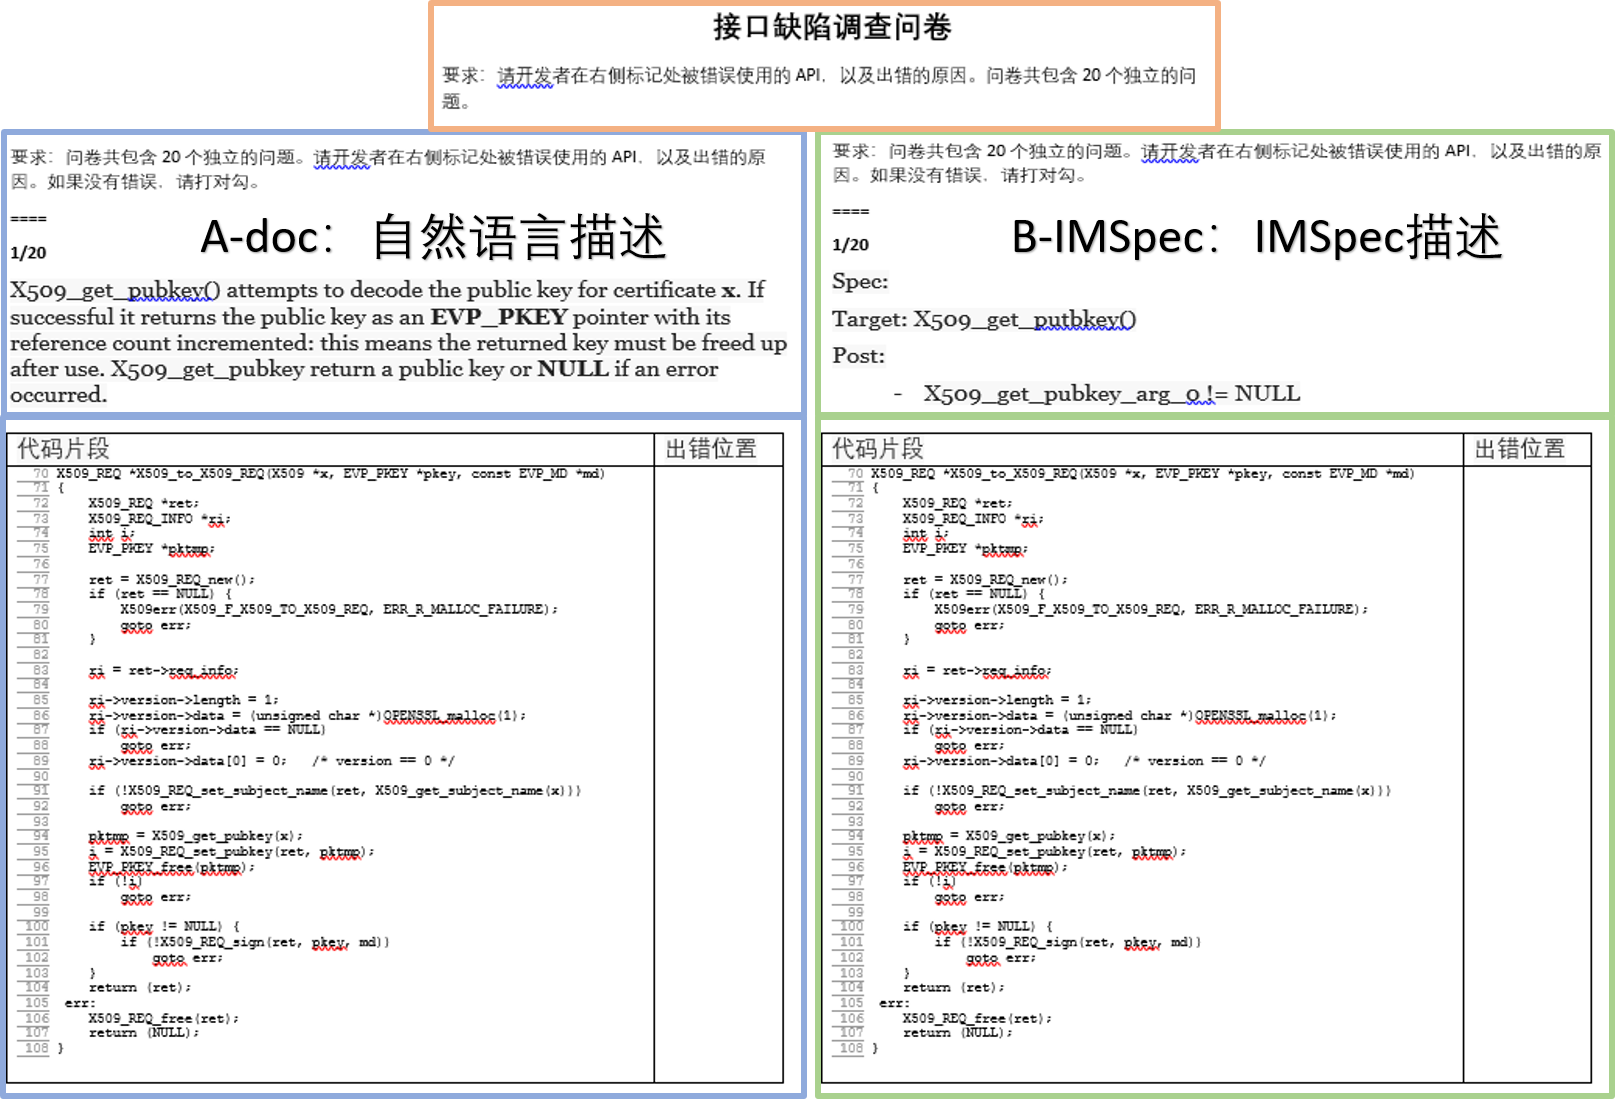
\includegraphics[width=0.85\linewidth]{figures/cp2-survey.png}
	\caption{
		接口误用缺陷检测调查问卷
	}
	\label{fig:2-5-survey}
\end{figure}

\paragraph{方法}
针对于“有效性”,本文以实际开发者作为评估对象,即通过实际开发者评估IMSpec是否能够有效地描述接口使用约束。
OpenSSL提供良好的接口使用用户手册~\footnote{https://www.openssl.org/docs/manmaster/man3/},
因此本文对OpenSSL的缺陷进行随机取样并用于评估。
在预实验中,作者对开发者一次能够接受的缺陷审查的数目进行调研。
结果显示5-10个是开发者能够接受的区间。
所以,本文将随机选择的10个缺陷实例与这些缺陷的修复版本随机排序,
并构造两组测试集:
A-doc组提供OpenSSL项目中基于自然语言描述的接口使用说明,
B-IMSpec提供基于IMSpec描述的接口使用约束条件。
通过随机选择的方式,每组测试集各发放给20名研究或者工作领域与测试、
程序分析等背景相关的实际开发人员。
对于A-doc组被测对象,作者对OpenSSL的背景进行介绍;
对于B-IMSpec组被测对象,作者对OpenSSL背景以及IMSpec进行简单的介绍。
特别地,为B-IMSpec组提供图\ref{fig:2-4-example}和图\ref{fig:2-4-example-imspec}作为参考资料。
本文请这些开发人员对代码中存在的缺陷进行标注,
如图\ref{fig:2-5-survey}中所示。
如果代码存在缺陷,请被测对象标注位置和原因;
如果没有则打对勾。
\begin{equation}
\label{eq:p}
P = \dfrac{\text{开发者报告中的真实缺陷数}}{\text{开发者报告缺陷总数}}
\end{equation}
\begin{equation}
\label{eq:r}
R = \dfrac{\text{开发者报告中的真实缺陷}}{10}
\end{equation}


令包含误用的测试用例为真实缺陷。
对于开发人员的标注结果,通过精度$P$和召回率$R$进行评估。
其中,精度的定义如公式\ref{eq:p}所示,
是被测对象找到缺陷中真实的缺陷个数与缺陷报告总数的比值。
较高的精度值表示缺陷检测效果误报率低,即找到的就是缺陷。
召回率的定义如公式\ref{eq:r}所示,是真实的缺陷与所有缺陷的商。
较高的召回率表示缺陷检测能力强、漏报率低,即能够找到更多缺陷。


\begin{table}[b]
	\centering
	\begin{minipage}[t]{\linewidth} % 如果想在表格中使用脚注,minipage是个不错的办法
		\caption{基于两种描述方式的开发者审查结果}
		\label{tab:2-5-survey}
			\begin{tabular}{ccccccccc}
			\hline
			\multirow{2}{*}{实验组} & \multicolumn{2}{c}{问卷情况} & \multicolumn{2}{c}{测试集} & \multicolumn{2}{c}{平局缺陷报告情况} & \multicolumn{2}{c}{平均结果} \\
			\cline{2-9}
			& 发放 & 收回 & 缺陷数& 正确数& 报告总数 & 真实缺陷 & $P$ & $R$ \\
			\hline
		A-doc	& 20 & 13 & 10& 10& 3.92 & 3.69 & 94.13\% & 36.90\% \\
		 B-IMSpec	& 20 & 18 & 10& 10& 8.06 & 7.94 & 98.51\% & 80.60\% \\
			\hline
		\end{tabular}
	\end{minipage}
\end{table}

\paragraph{结果}
本文将针对于有效性的评估结果展示在表\ref{tab:2-5-survey}中。
在所有发放的调查问卷中,A-doc组共收回13份(65\%),
B-IMSpec组共收回18份(90\%)。
在问卷中,共包含10个正确的使用和10个错误的使用。
本文对收到的调查问卷中所有缺陷报告进行统计。
特别地,对于问卷中没有做出标记的用例,
本文认为是开发者没有能够找到该缺陷,
即认为是正确使用效果等同于对勾。
如表中所示,A-doc组平均报告缺陷总数为3.92个,其中3.69个为真实缺陷;
B-IMSpec组平均报告缺陷总数为8.06个,其中7.94个为真实缺陷。
在统计后,本文对两组的开发者进行二次回访,
对没有回复的原因、缺陷定位的方法、误报和漏报的原因、缺陷分析中遇到的困难、
与自然语言相比IMSpec是否能够对接口使用约束描述更有效等问题进行调研。
在分析和比对后,本文将结果总结如下。

{\kaishu 精度与召回率 }
如表\ref{tab:2-5-survey}中所示,两组的精度都很高。
其中A-Doc组的平均检测精度为94.13\%,B-IMSpec的平均检测精度为98.51\%。
该结果显示,测试人员对于自然语言和IMSpec都能够正确理解,
即两者对接口使用约束条件的描述能力相同。
然而两组的召回率却存在较大差异,
其中A-doc组的召回率为36.9\%,比B-IMSpec组低43.7\%。
在对调查问卷本身和二次回访的结果进行分析和总结后,
本文发现A-doc组13个返回结果的被测对象中有10个并没有完全进行,
即其后几个缺陷没有做出标记,也没有打对勾或者提供任何正确使用的标记。
该现象的一个主要原因是,测试人员对自然语言的描述失去耐心。
在二次回访中,作者将基于IMSpec描述发送给这些被测对象。
结果显示,开发者相比于自然语言,更愿意接受类程序语言的IMSpec。
因此,相对于自然语言,开发者认为IMSpec的描述有效性更好。
	
{\kaishu 被测对象遇到的困难 }
本文对被测对象遇到的困难、误报漏报的原因进行分析和总结。
结果显示,开发者在进行调研问卷的过程中,存在如下几个主要困难:
\begin{enumerate}
	\item 时间问题。
	在二次回访的过程中,A-doc组中有3位第一次没有回复的开发者解释,
	他们忽略该调研的主要原因有两个。
	一方面,20个测试用例太多,测试者认为需要大量的时间进行分析。
	另一方面,当看到自然语言描述的规约时,测试者产生放弃进行测试的想法。
	\item 结果不一致。
	在两组测试人员当中,绝大部分被测对象没有OpenSSL的开发经验。
	但是在提供接口使用约束的条件后,
	开发者能够对这些领域相关的API进行缺陷检测。
	然而,被测对象的结果存在两方面的不一致。
	一方面,同一个开发人员对于同种缺陷模式,
	有的成功找到缺陷位置和原因,有的则没有找到。
	另一方面,同一个缺陷,有的开发者认为是缺陷有的则认为不是缺陷。
	特别地,对于参数检查问题,不同的开发者理解不同,
	即有的认为必须进行检查有的认为可以不检查。
	\item 上下文信息不足。
	为节省篇幅以及对问卷长度的担心,
	本文每个测试用例只提供目标API的单层函数的代码。
	特别地,对于长度过长的调用,进行程序截取。
	因此,两组测试人员都表示,很多情况下缺失的上下文信息会影响结果的判断。
	该影响主要表现在召回率上。
\end{enumerate}
	
针对于IMSpec描述的有效性,
评估结果显示实际开发者通该语言能够有效地理解接口使用约束。
同时,评估结果显示相对于自然语言,
IMSpec的表现形式更利于开发者理解接口使用约束。

\section{本章小结}
\label{sec:2.6}
本章提出基于缺陷模式的C程序接口使用约束领域特定语言。
为有效地进行语言设计,本章首先对C程序中接口误用缺陷实例进行研究和总结。
以不同领域、广泛使用的六个开源软件作为研究对象,
对开发过程中出现的830个实际接口误用缺陷实例进行分析和归纳。
本章总结出三类常见接口误用缺陷模式,包括:
不正确的参数使用、不正确的异常处理以及不正确的因果调用关系。
这些缺陷模式有利于研究人员和开发者理解API误用缺陷的本质,
设计和开发更好的API、接口缺陷检测工具。
基于常见缺陷模式,
本章提出IMSpec领域特定语言,以描述C程序中接口使用约束,
并给出该语言的设计动机、语法结构和形式语义。
本章将IMSpec应用于实际项目的缺陷实例中,
应用结果显示该语言能够有效地描述实际项目中接口使用约束。
